\documentclass[12pt]{article}
\usepackage[utf8]{inputenc}
\usepackage[left=2cm,right=2cm,top=2cm,bottom=2cm]{geometry}
\usepackage{graphicx, amsmath, listings, xcolor}
\usepackage[small]{caption}
\usepackage{subcaption}
\usepackage[spanish]{babel}
\usepackage{url}
\setlength{\parskip}{\baselineskip}
\graphicspath{ {images/} }
\spanishdecimal{.}

\usepackage{hyperref}
\hypersetup{
	colorlinks=true,
	linkcolor=blue,     
	urlcolor=blue,
	citecolor=blue,
}

\definecolor{dkgreen}{rgb}{0,0.6,0}
\definecolor{gray}{rgb}{0.5,0.5,0.5}
\definecolor{mauve}{rgb}{0.58,0,0.82}

\lstset{frame=none,
	language=Python,
	aboveskip=3mm,
	belowskip=3mm,
	showstringspaces=false,
	columns=flexible,
	basicstyle={\small\ttfamily},
	numbers=none,
	numberstyle=\tiny\color{gray},
	keywordstyle=\color{blue},
	commentstyle=\color{dkgreen},
	stringstyle=\color{mauve},
	breaklines=true,
	breakatwhitespace=true,
	tabsize=3
}

\begin{document}


	\thispagestyle{empty}

	\begin{center}
		{\Large \bf Distribución normal y generación pseudoaleatoria}\\
		Gabriela S\'anchez Y.\\
		5064
	\end{center}
 
	En el presente trabajo se realiza un estudio del generador lineal congruencial \cite{wiki_lcg}, algoritmo que permite obtener una secuencia de números pseudoaleatorios y el método de Box-Muller \cite{wiki_bmt}, un método de generación de números con distribución normal. Además se hace analiza el efecto que tiene el usa del generador lineal congruencial en la generación de los números del método de Box-Muller. La experimentación se realiza con la ayuda del lenguaje de programación \textsc{R} versión 4.0.2 \cite{r}. El código puede encontrarse en el archivo \texttt{t5.R} \cite{mpa_gaby}.


	\section{Generador lineal congruencial}
	
	El generador lineal congruencial es un algoritmo que permite obtener una secuencia de números pseudoaleatorios mediante la relación de recurrencia (\ref{ec_recurrencia}), donde $m$ es el módulo, $a$ el multiplicador, $c$ el incremento y $X_0$ la semilla o valor inicial. Por lo tanto para poder obtener la secuencia son necesarios estos cuatro parámetros. 
	\begin{equation}
	X_{n+1} = \left(a\cdot X_n + c \right) \, \textup{mod} \, m.
	\label{ec_recurrencia}
	\end{equation}
	
	Es claro que esta relación permitirá generar a lo más $m-1$ valores diferentes, pero si no se eligen bien los coeficientes $a$ y $c$ el número se reduce.
	
	Un primer experimento analiza el efecto de usar solo números primos de uno, dos, tres y cuatro dígitos en los parámetros. Con excepción de los primos de un dígito, todos los demás se eligieron de forma ``aleatoria''. Considerando una semilla $X_0 = 103$ se generan secuencias de $n=1000$ números y se verifica con la prueba de {\em Shapiro} si cumplen con la uniformidad o no. En el cuadro \ref{resultados_primos} se muestran los resultados que se obtienen del $p$-valor al realizar la prueba y el periodo que se logra con la configuración.
	
	\begin{table}[b]
		\centering
		\caption{Resultados obtenidos en el periodo y $p$-valor para las diferentes configuraciones de parámetros.}
		\label{resultados_primos}
		\begin{tabular}{lrr}
			\hline
			Parámetros $a, c, m$ & $p$-valor & Periodo\\
			\hline
			3, 5, 7 & 0 & 6 \\
			11, 43, 97 & 7.495585e-72 & 48 \\
			59, 43, 97 & 0.12690289 & 96 \\
			613, 919, 857 & 0.3345382 & 428 \\
			1291, 3821, 5449 & 0.71023907  & 1816 \\
			\hline
		\end{tabular}
	\end{table}

	La primera configuración de parámetros genera una secuencia con un periodo muy pequeño, es decir, la secuencia solo tiene seis valores diferentes por lo que no es de extrañar que no pase la prueba de normalidad. Un caso interesante es la segunda y tercera configuración, aunque el módulo y el incremento son primos entre sí en ambos casos, la variación en el valor del multiplicador tiene un efecto considerable en la secuencia que se genera. Nótese que con $a=11$ la secuencia logra un periodo de 48 mientras que con $a=59$ alcanza el periodo máximo, lo que le permite pasar la prueba de {\em Shapiro}.
	
	Con estos resultados se puede concluir que el método es bastante sensible a los parámetros para el módulo, multiplicador e incremento. ¿Qué pasa si se varía el valor de la semilla? ¿qué efecto tiene?.
	
	Utilizando las segunda, tercera y cuarta configuración mostradas en el cuadro \ref{resultados_primos}, ahora se varía el valor de la semilla en 5, 59, 103 y 1117, también números primos elegidos al ``azar'', para analizar el efecto que tiene en la generación de la secuencia.
	
	La figura \ref{varia_semilla} muestra la distribución de los valores generados. A simple vista no se observa mucha diferencia al variar el valor de la semilla, con excepción de la configuración $a=11$, $c= 43$ y $m=97$. Aunque es importante recordar que la configuración no crea una buena secuencia (en términos de uniformidad). La figura permite corroborar el resultado previamente obtenido con la prueba de uniformidad, los valores no parecen distribuirse de manera uniforme.
	
	\begin{figure}
		\begin{subfigure}{\textwidth}
			\centering
			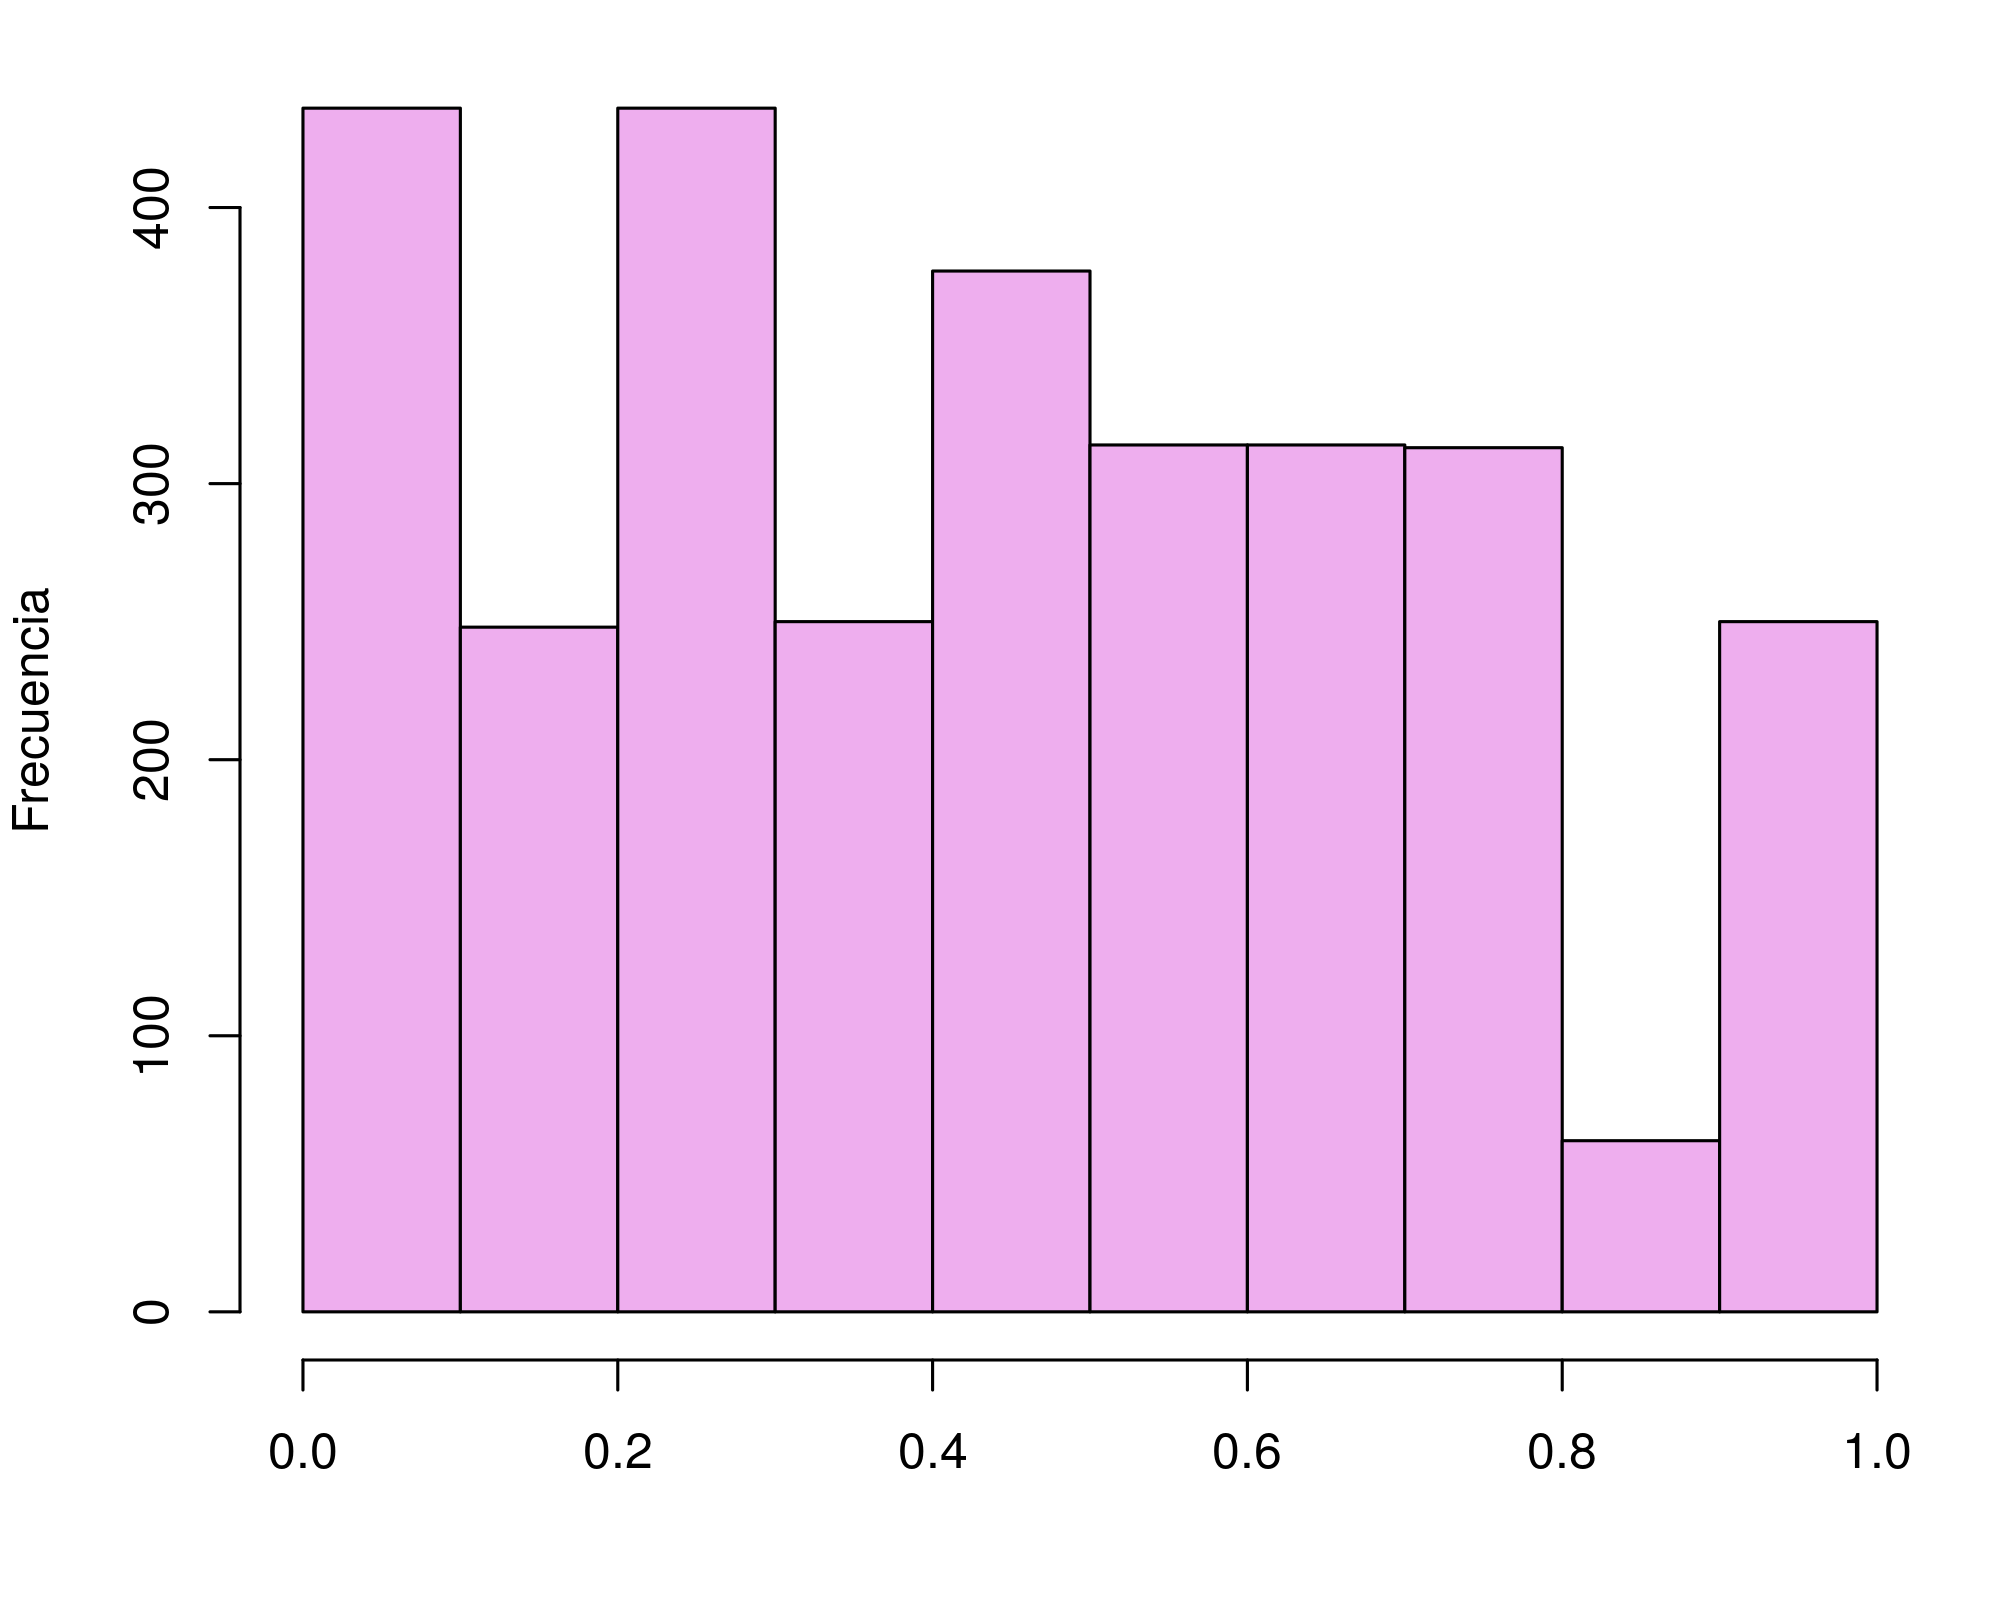
\includegraphics[scale=0.34]{hist_5-11-43-97.png}
			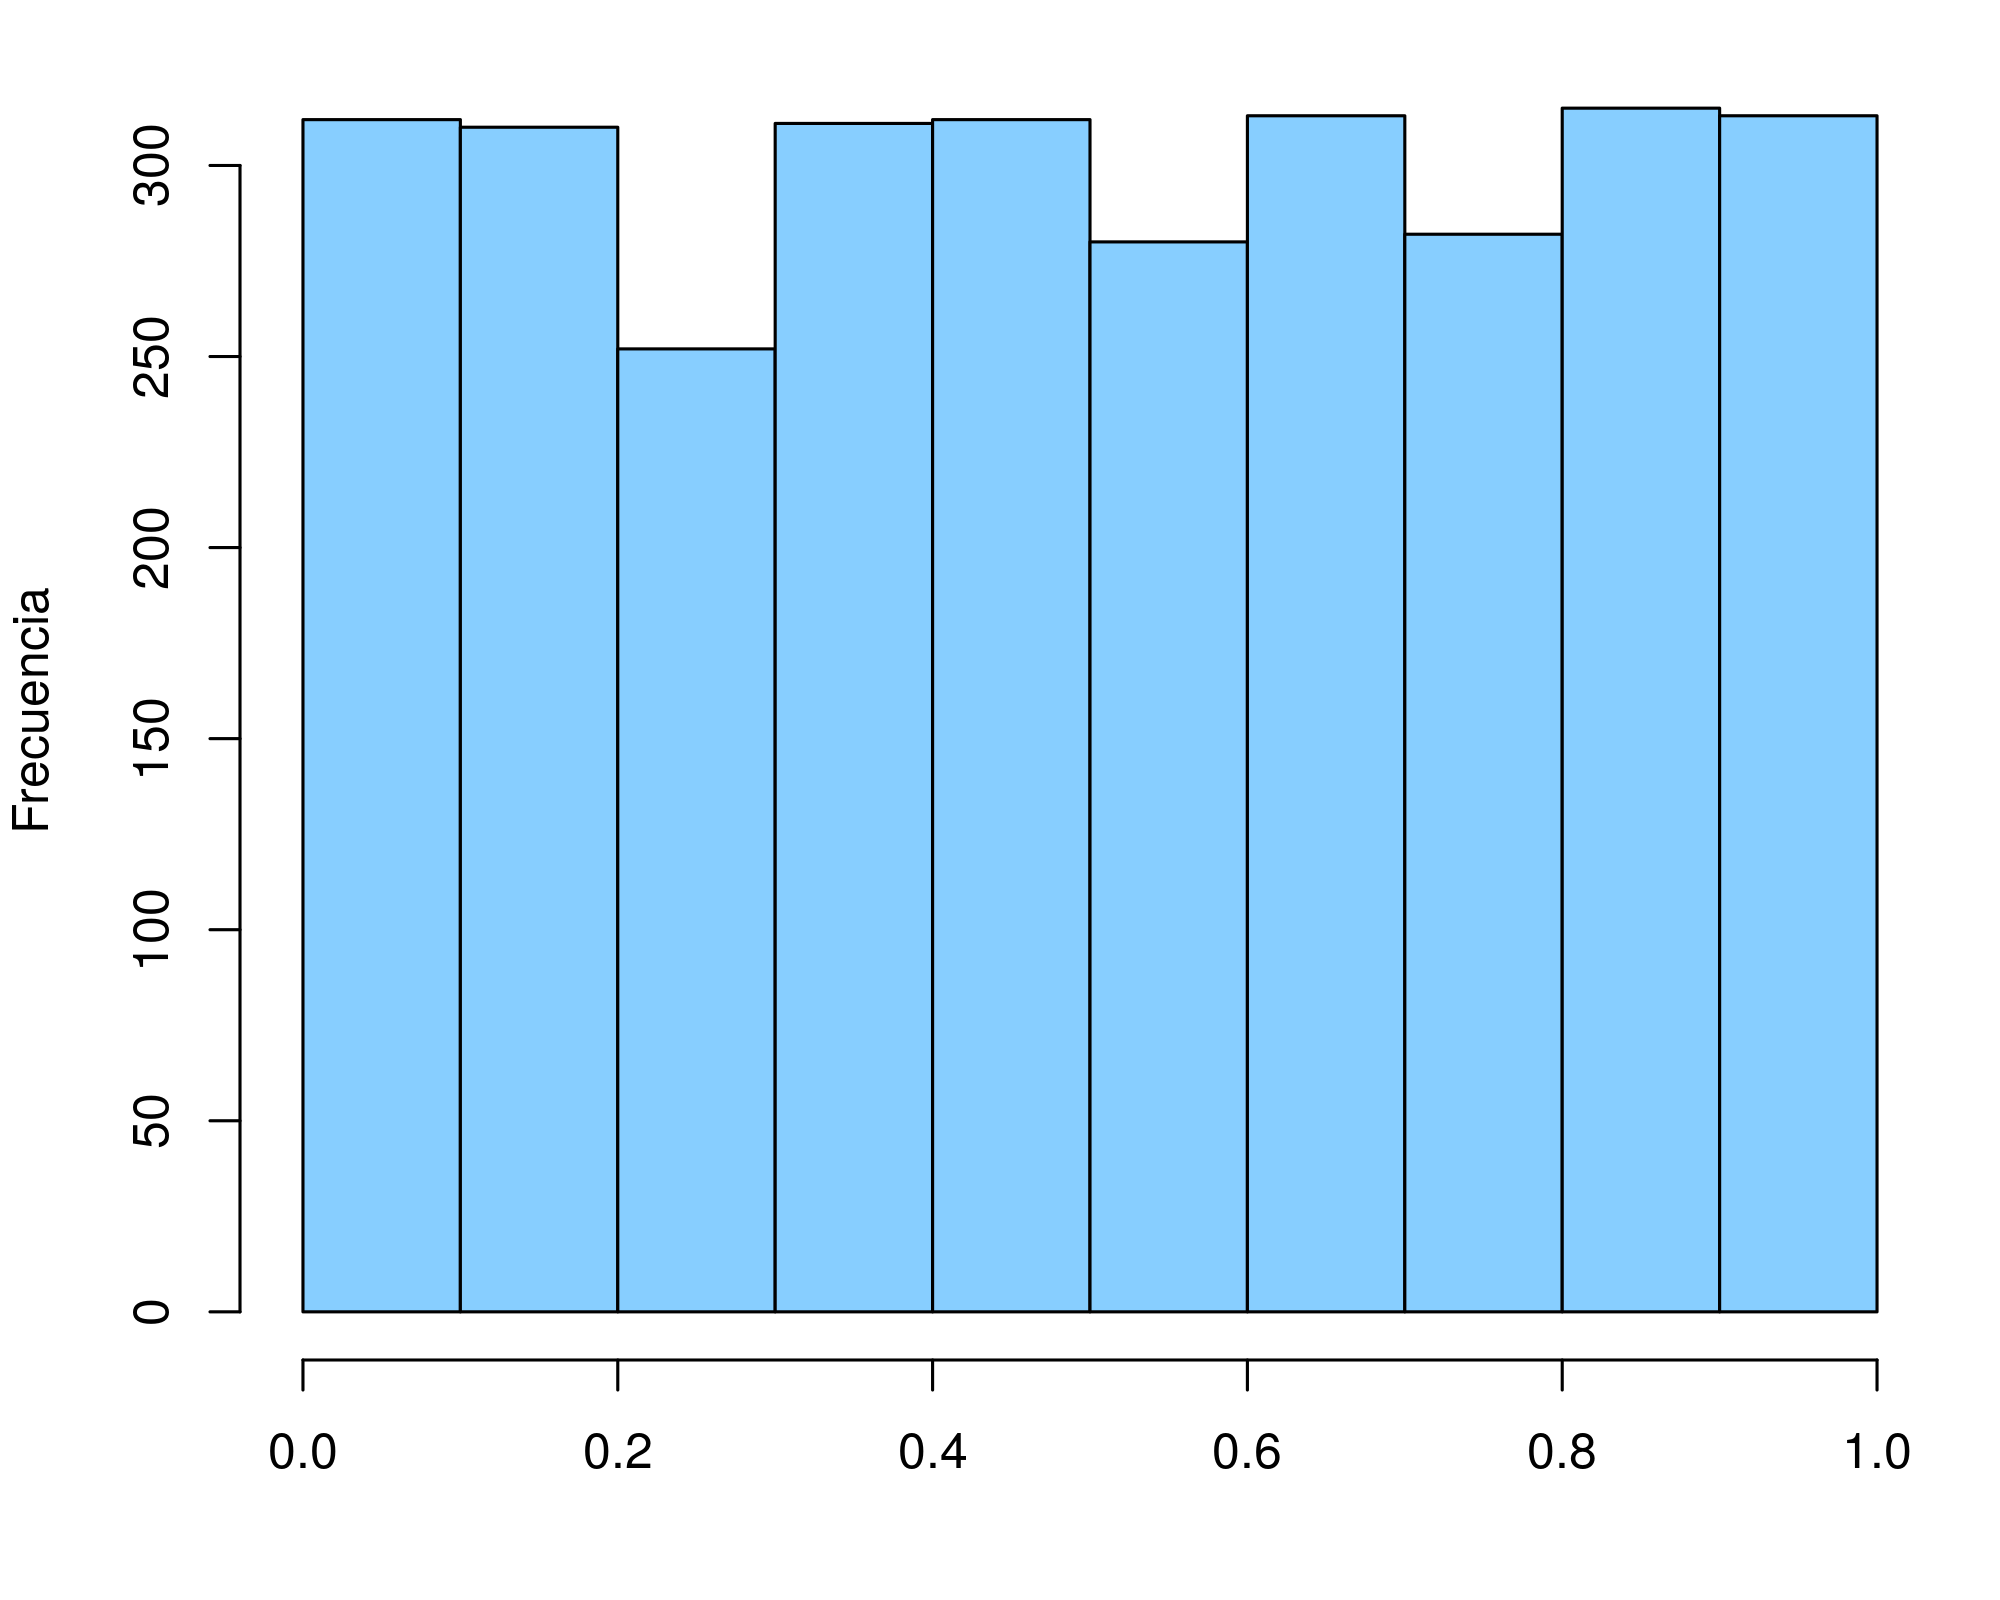
\includegraphics[scale=0.34]{hist_5-59-43-97.png}
			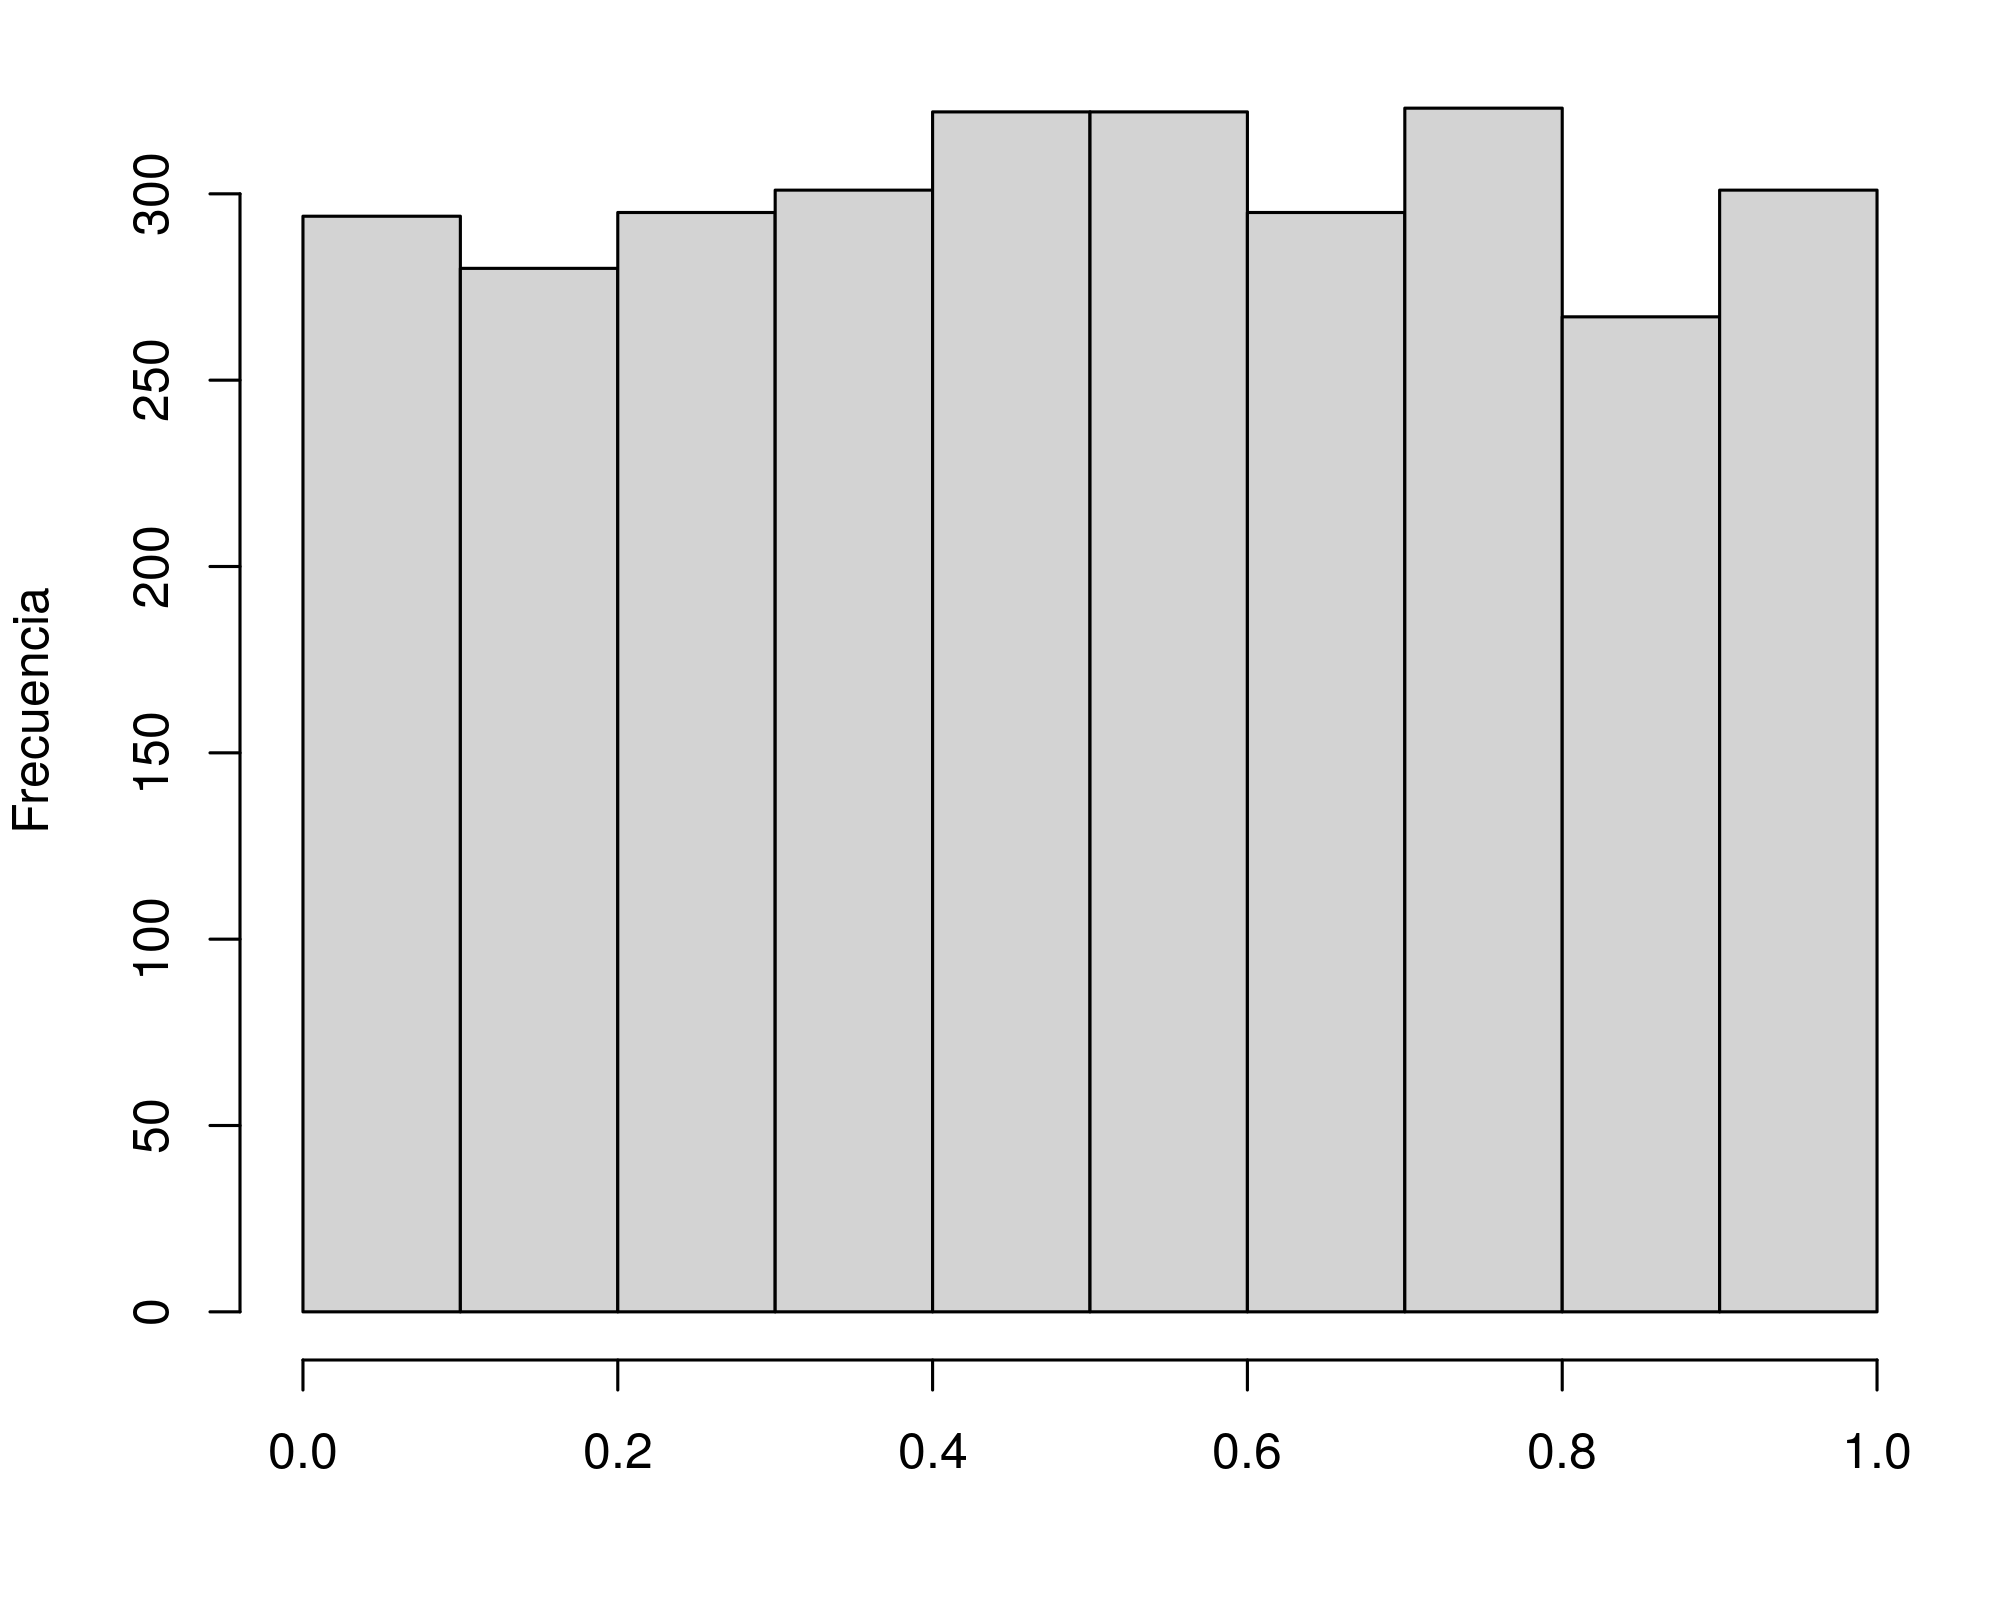
\includegraphics[scale=0.34]{hist_5-613-919-857.png}
			\caption{$X_0 = 5$.}
			\label{semilla5}
		\end{subfigure}
		\begin{subfigure}{\textwidth}
			\centering
			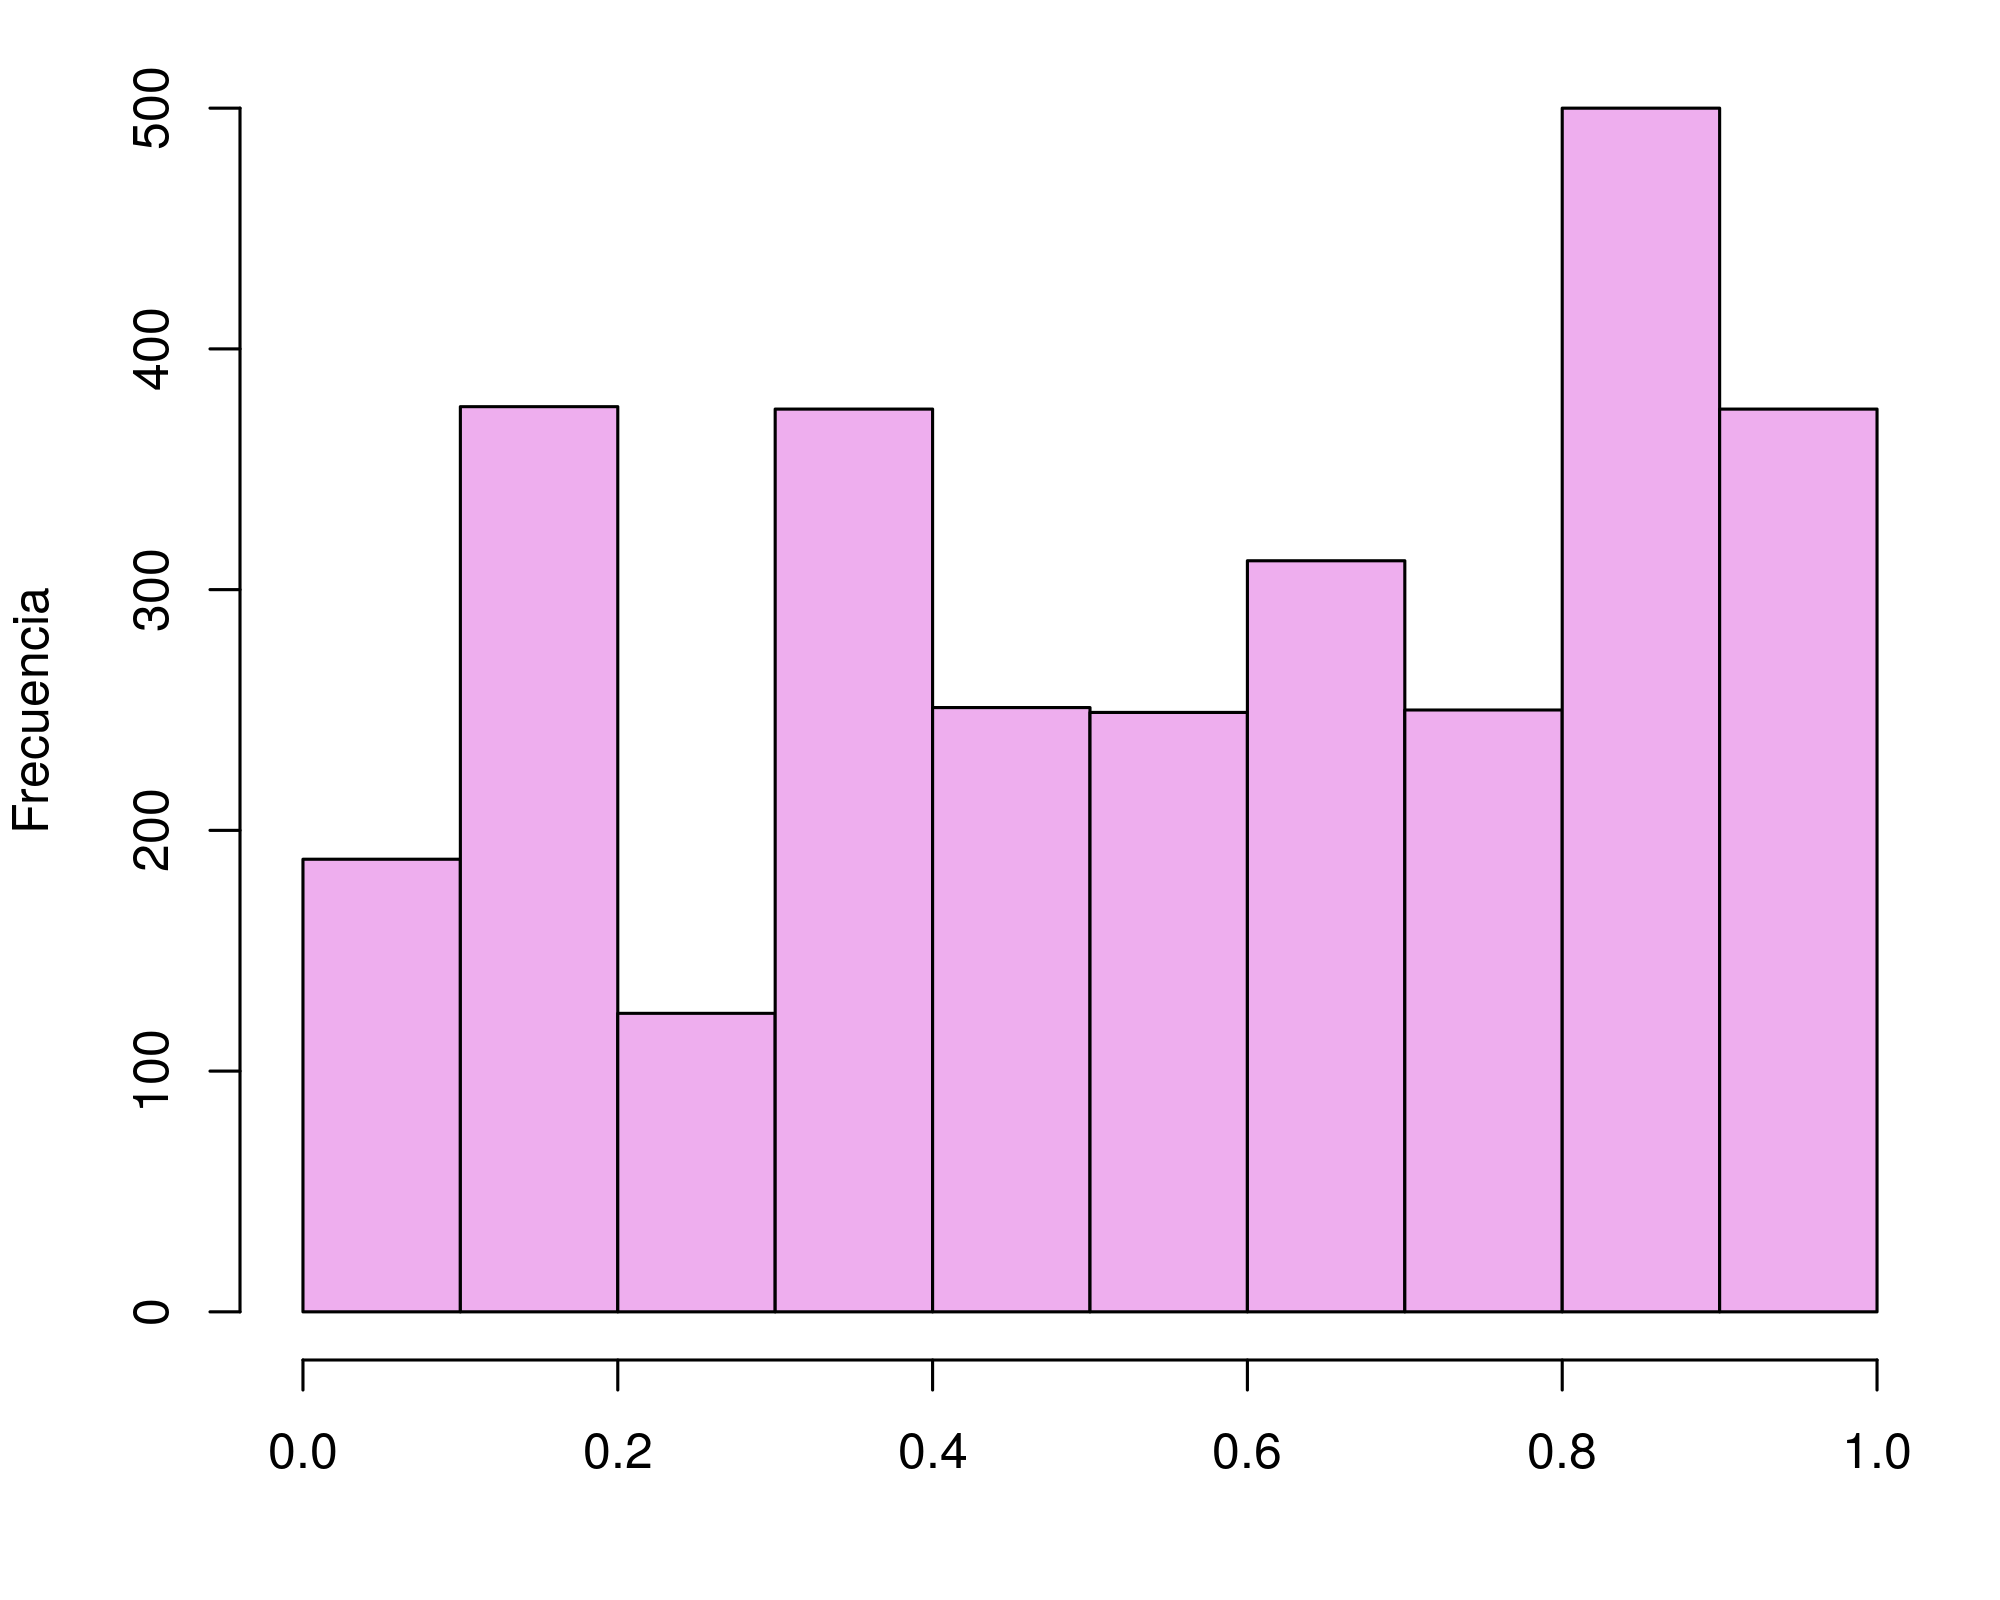
\includegraphics[scale=0.34]{hist_59-11-43-97.png}
			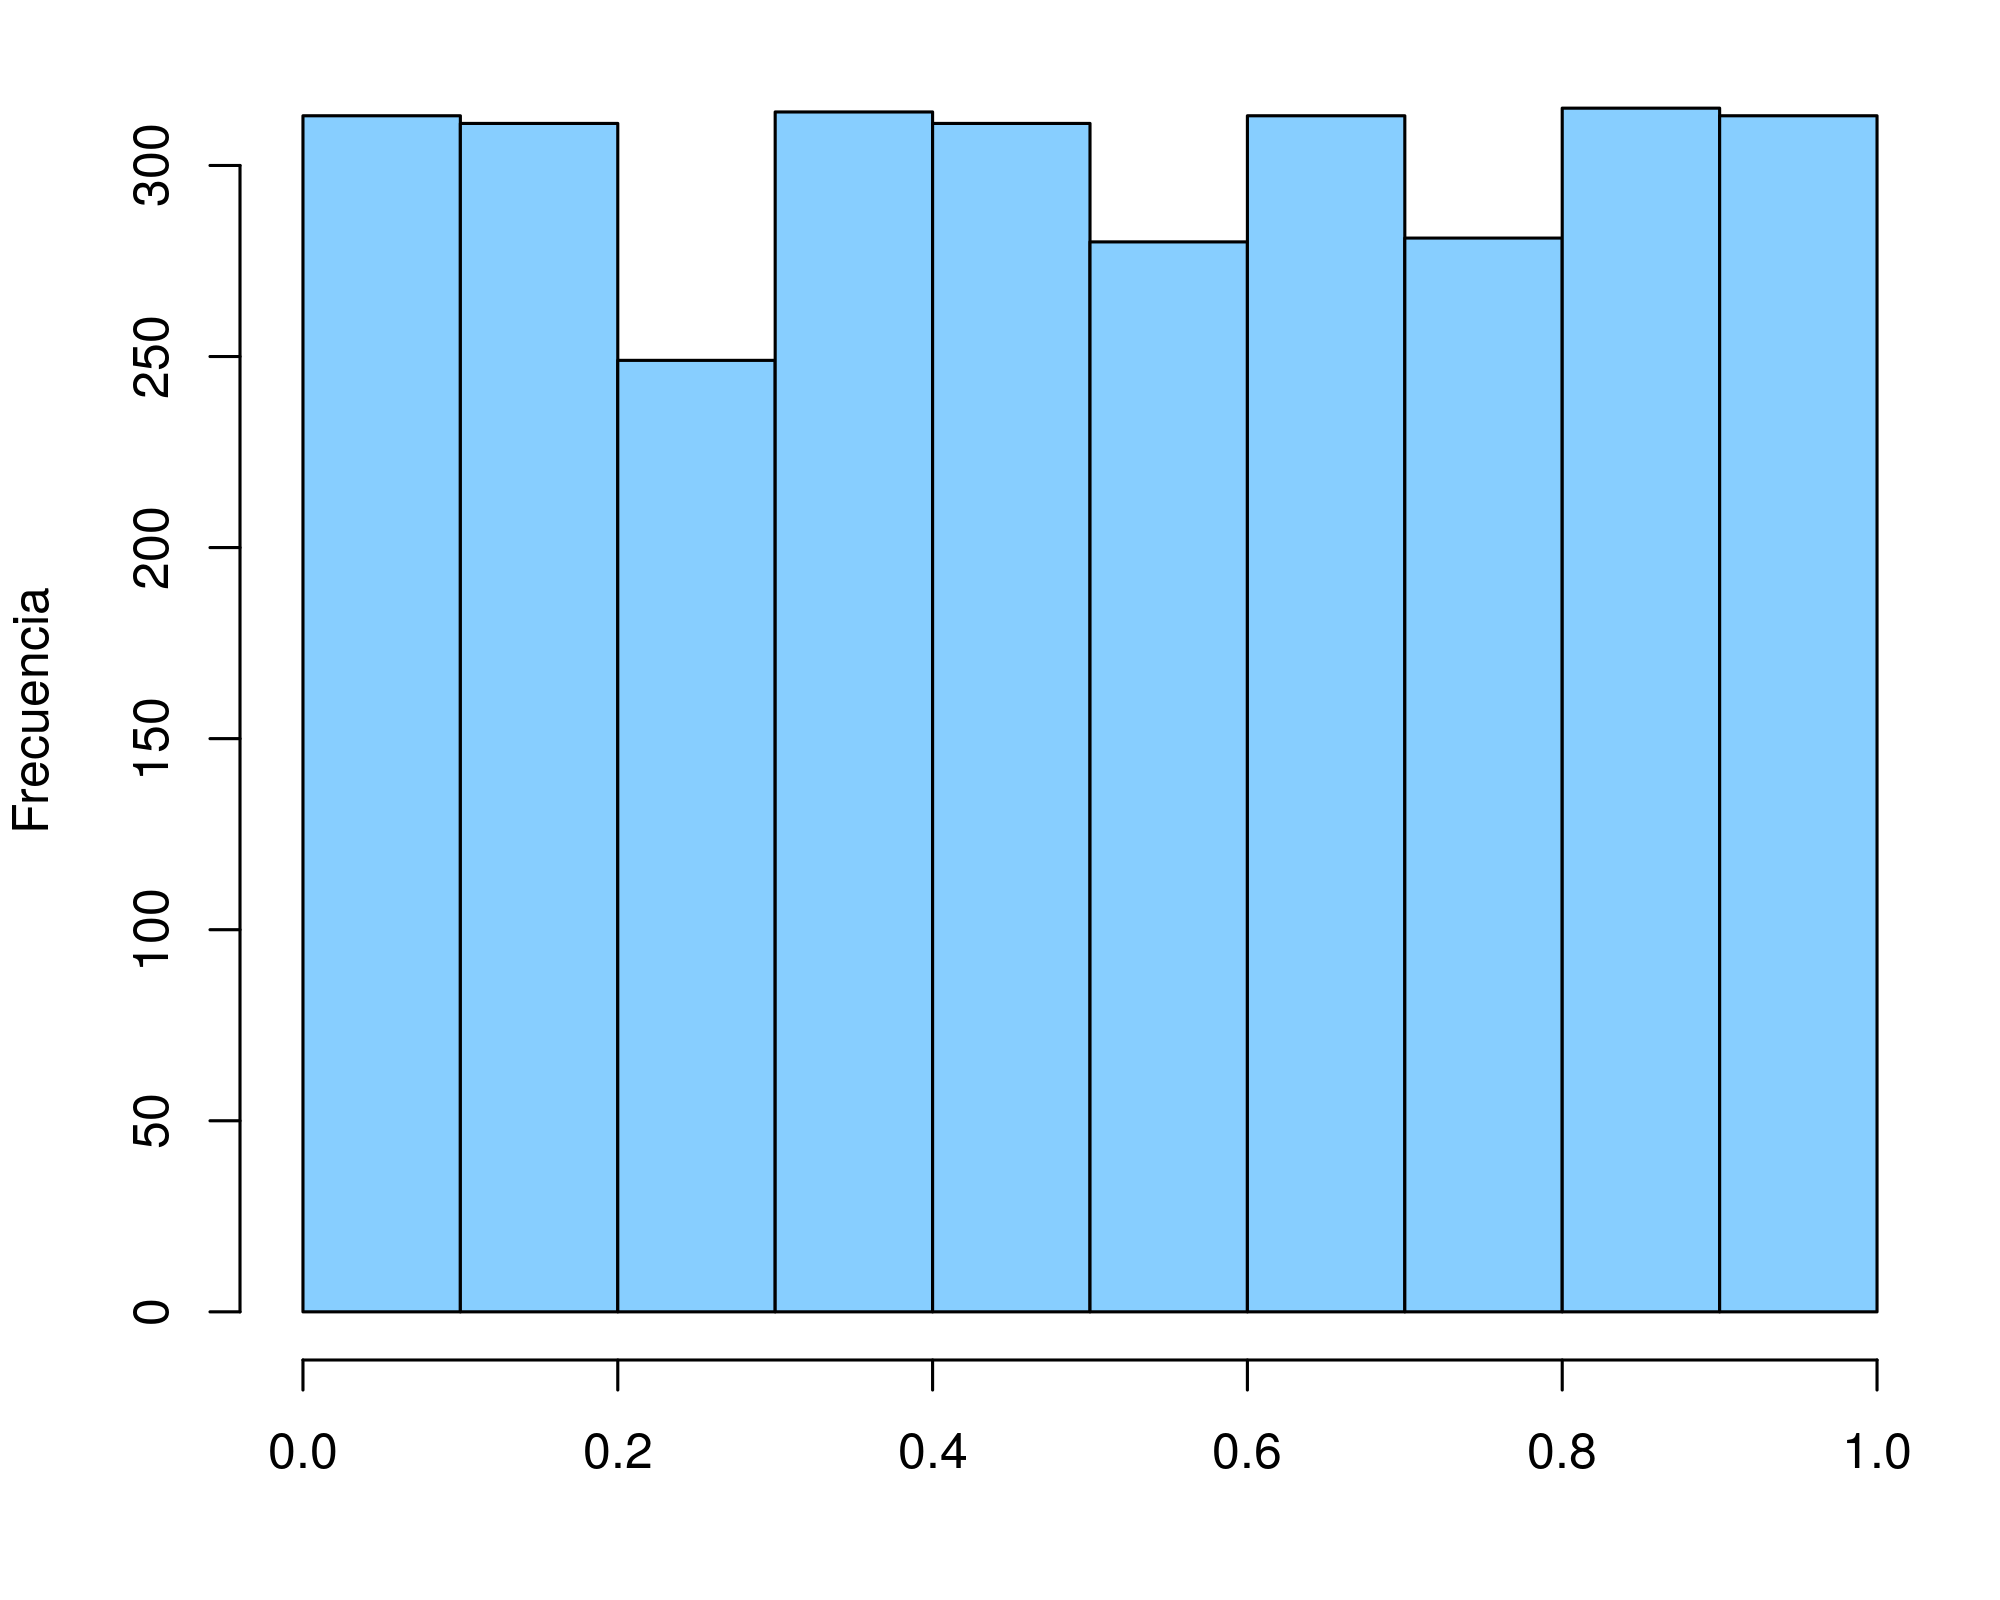
\includegraphics[scale=0.34]{hist_59-59-43-97.png}
			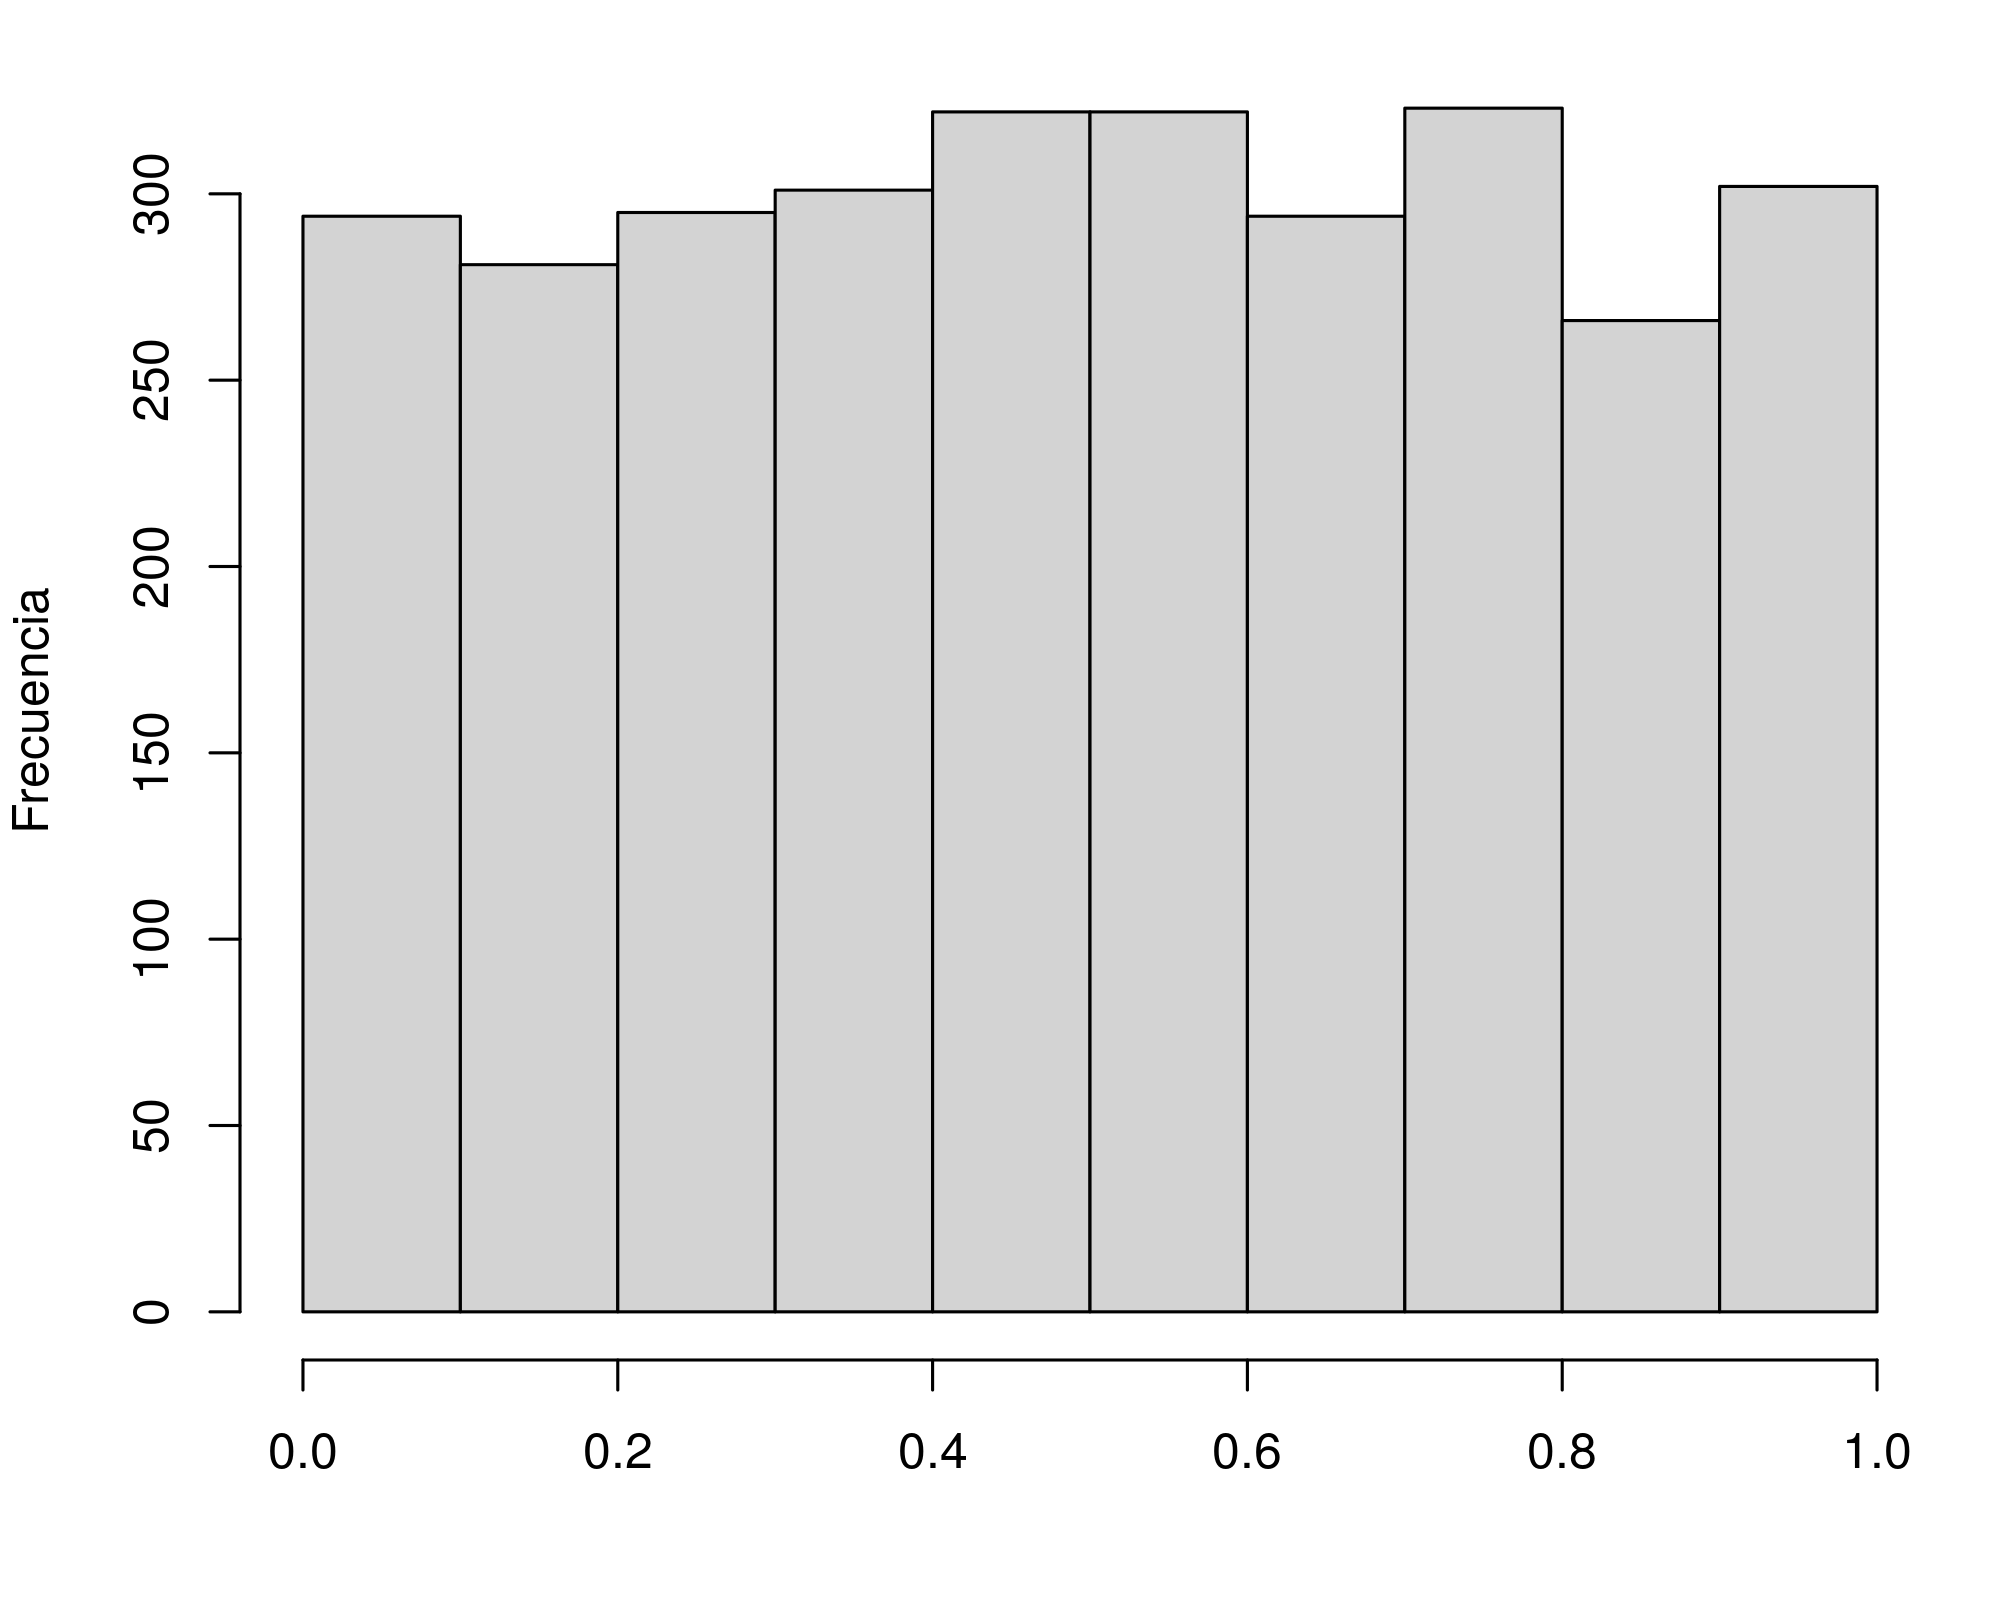
\includegraphics[scale=0.34]{hist_59-613-919-857.png}
			\caption{$X_0 = 59$.}
			\label{semilla59}
		\end{subfigure}
		\begin{subfigure}{\textwidth}
			\centering
			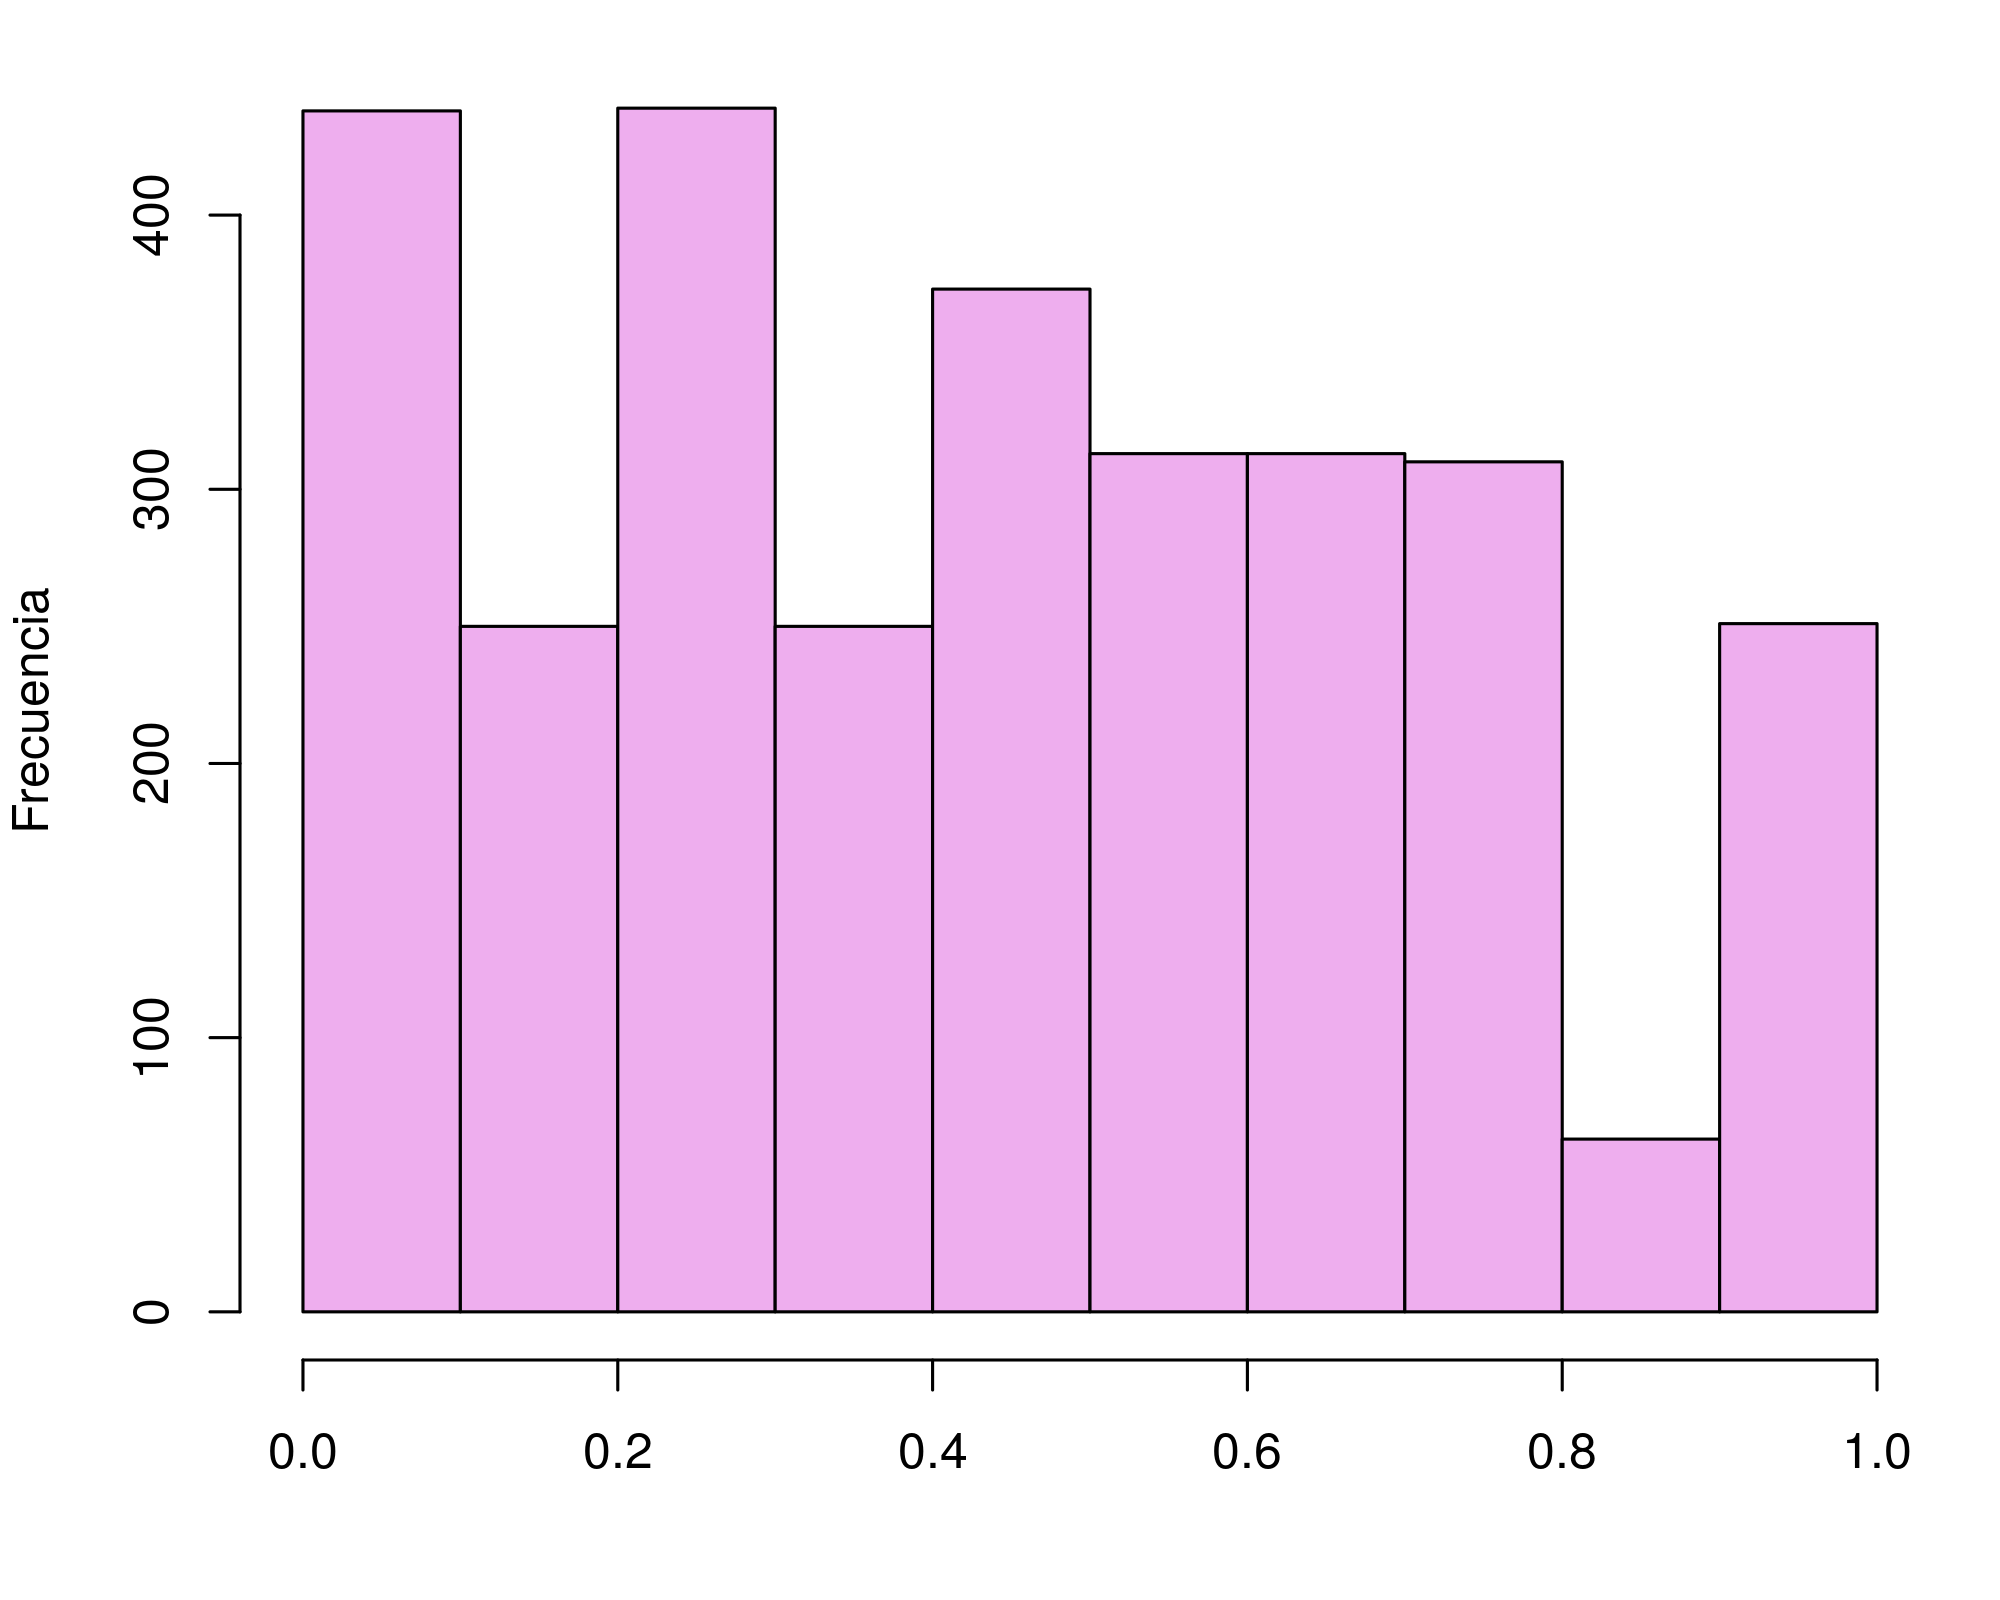
\includegraphics[scale=0.34]{hist_103-11-43-97.png}
			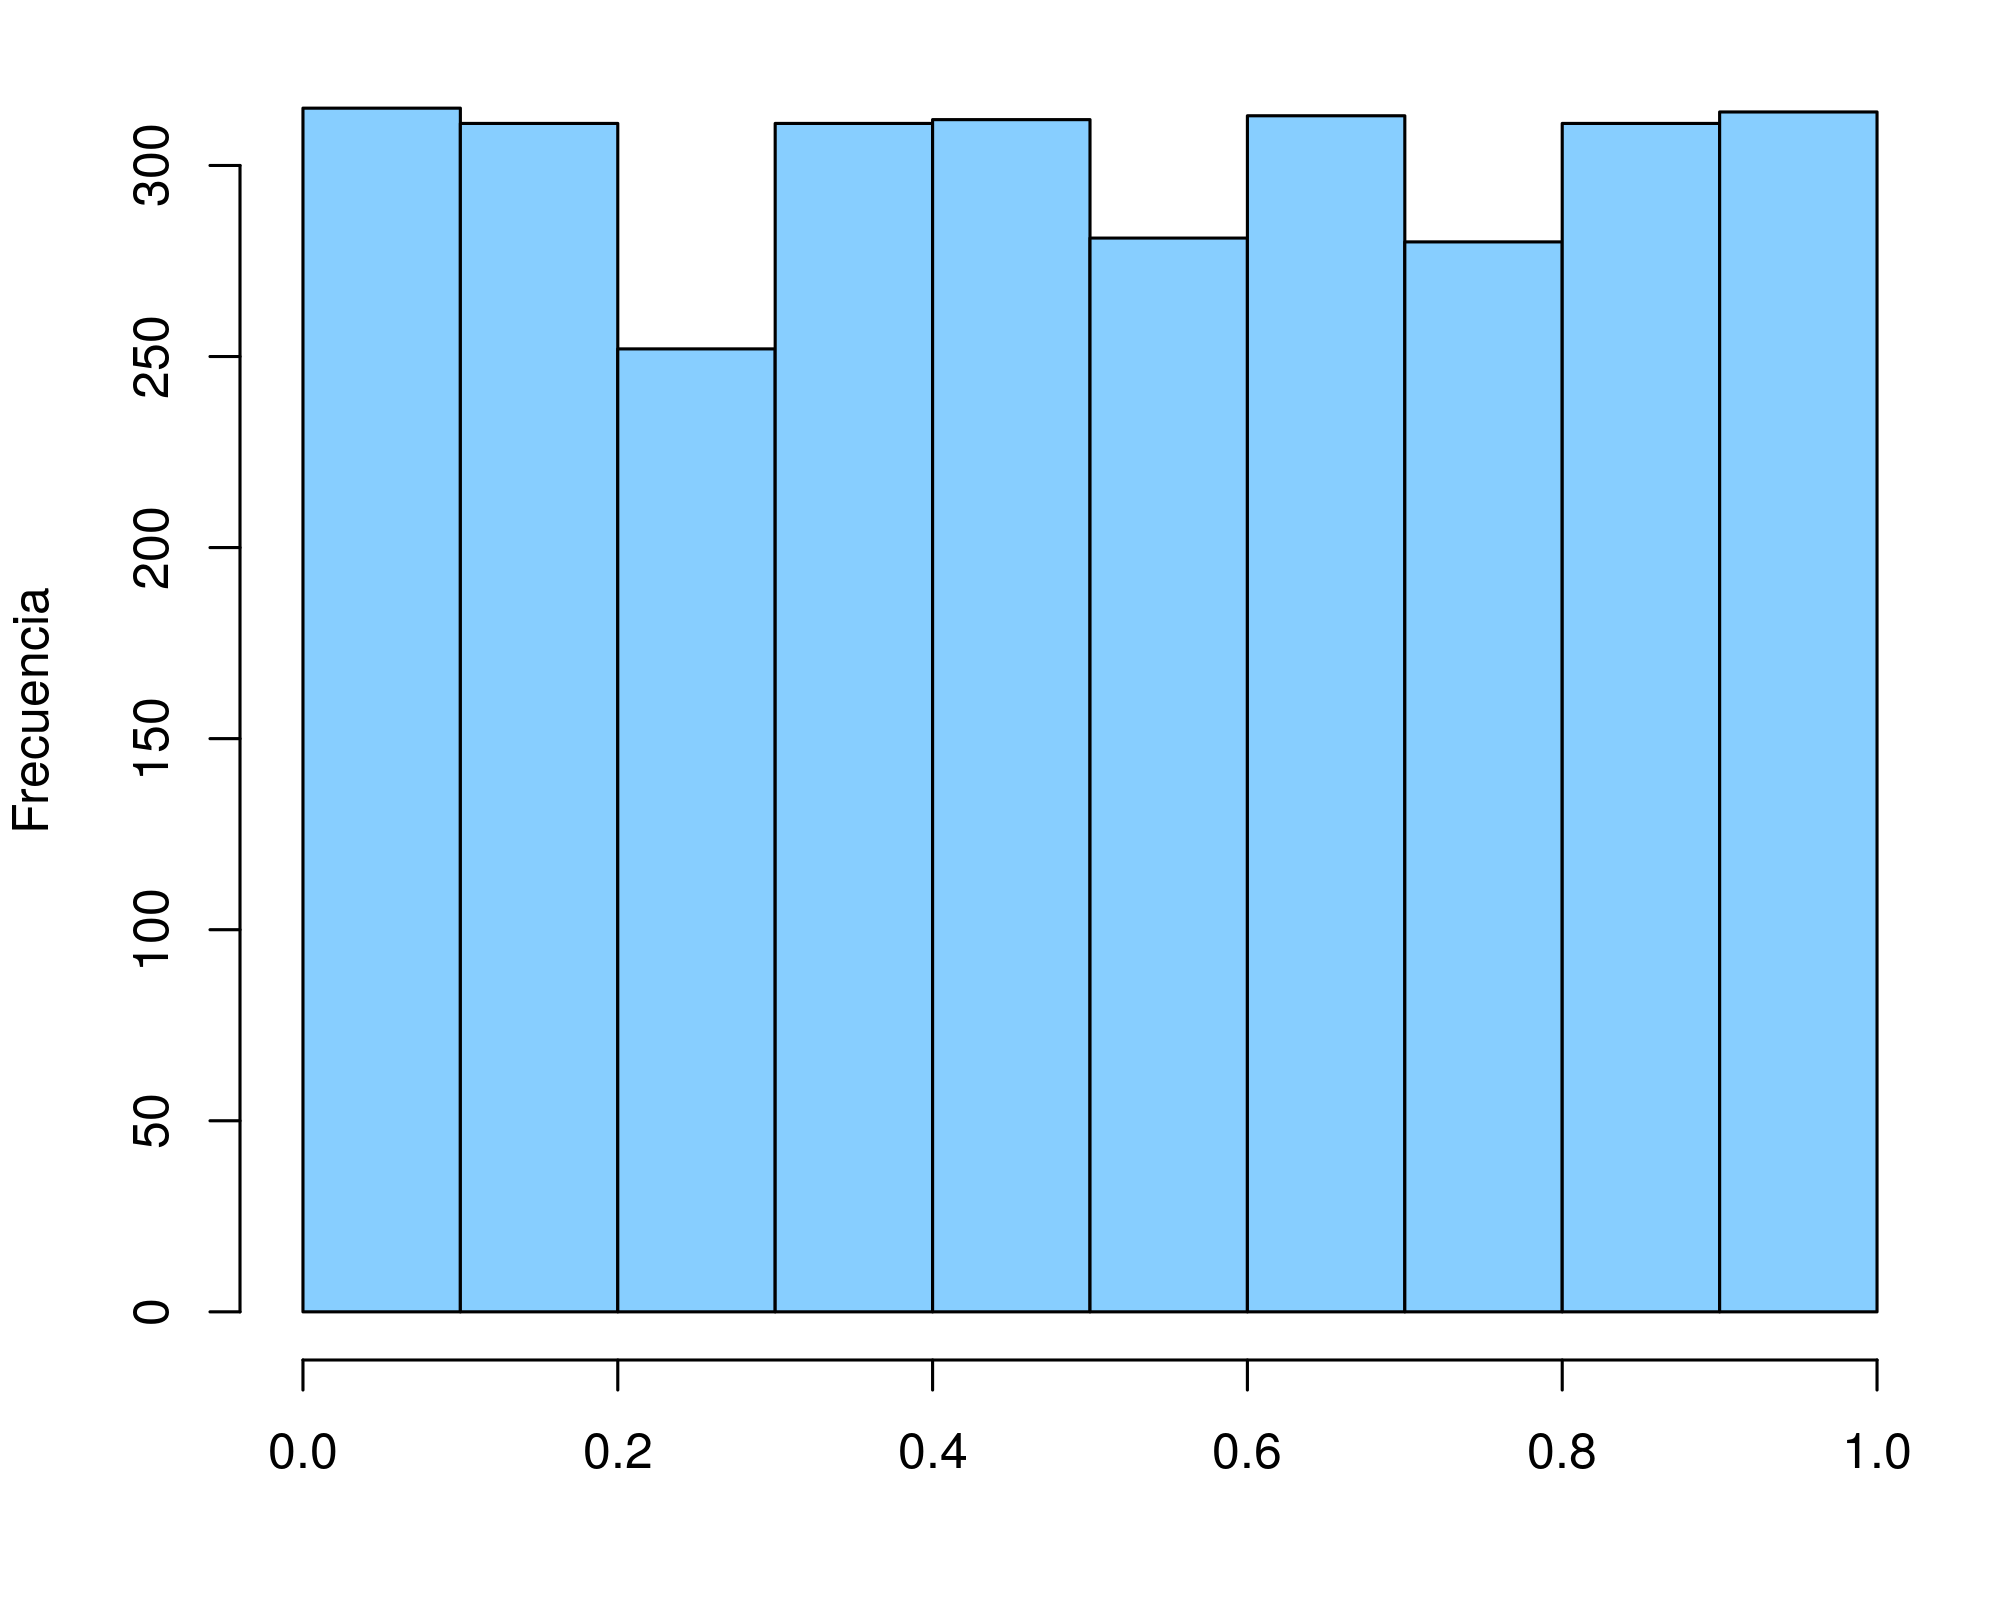
\includegraphics[scale=0.34]{hist_103-59-43-97.png}
			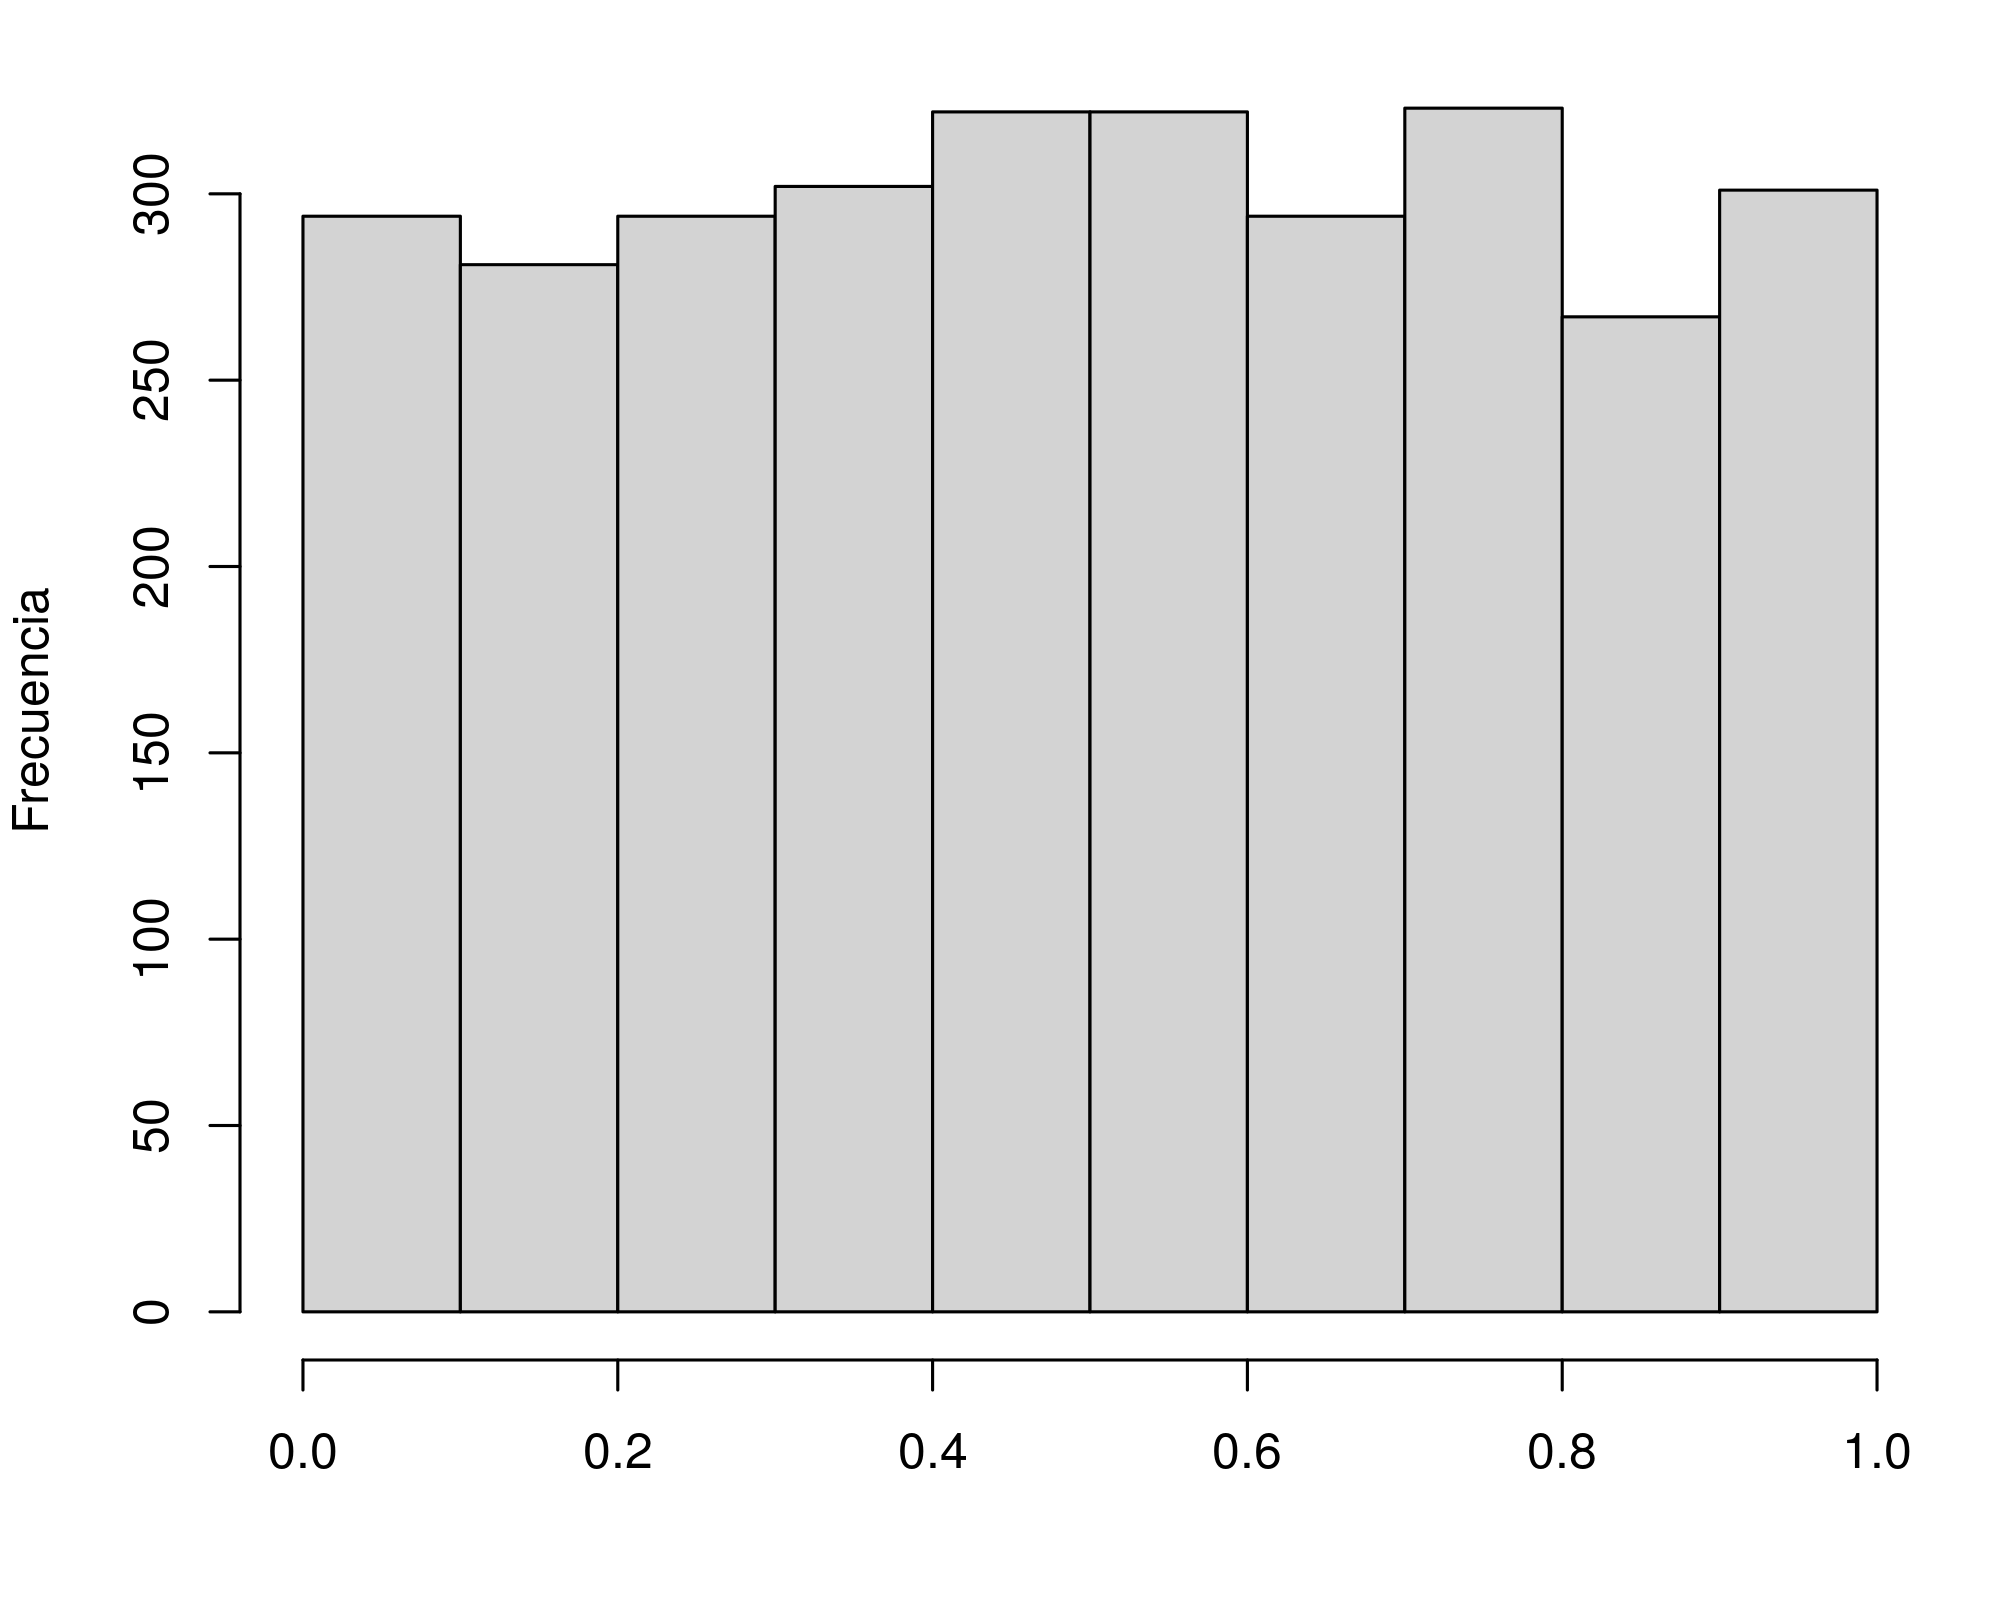
\includegraphics[scale=0.34]{hist_103-613-919-857.png}
			\caption{$X_0 = 103$.}
			\label{semilla103}
		\end{subfigure}
		\begin{subfigure}{\textwidth}
			\centering
			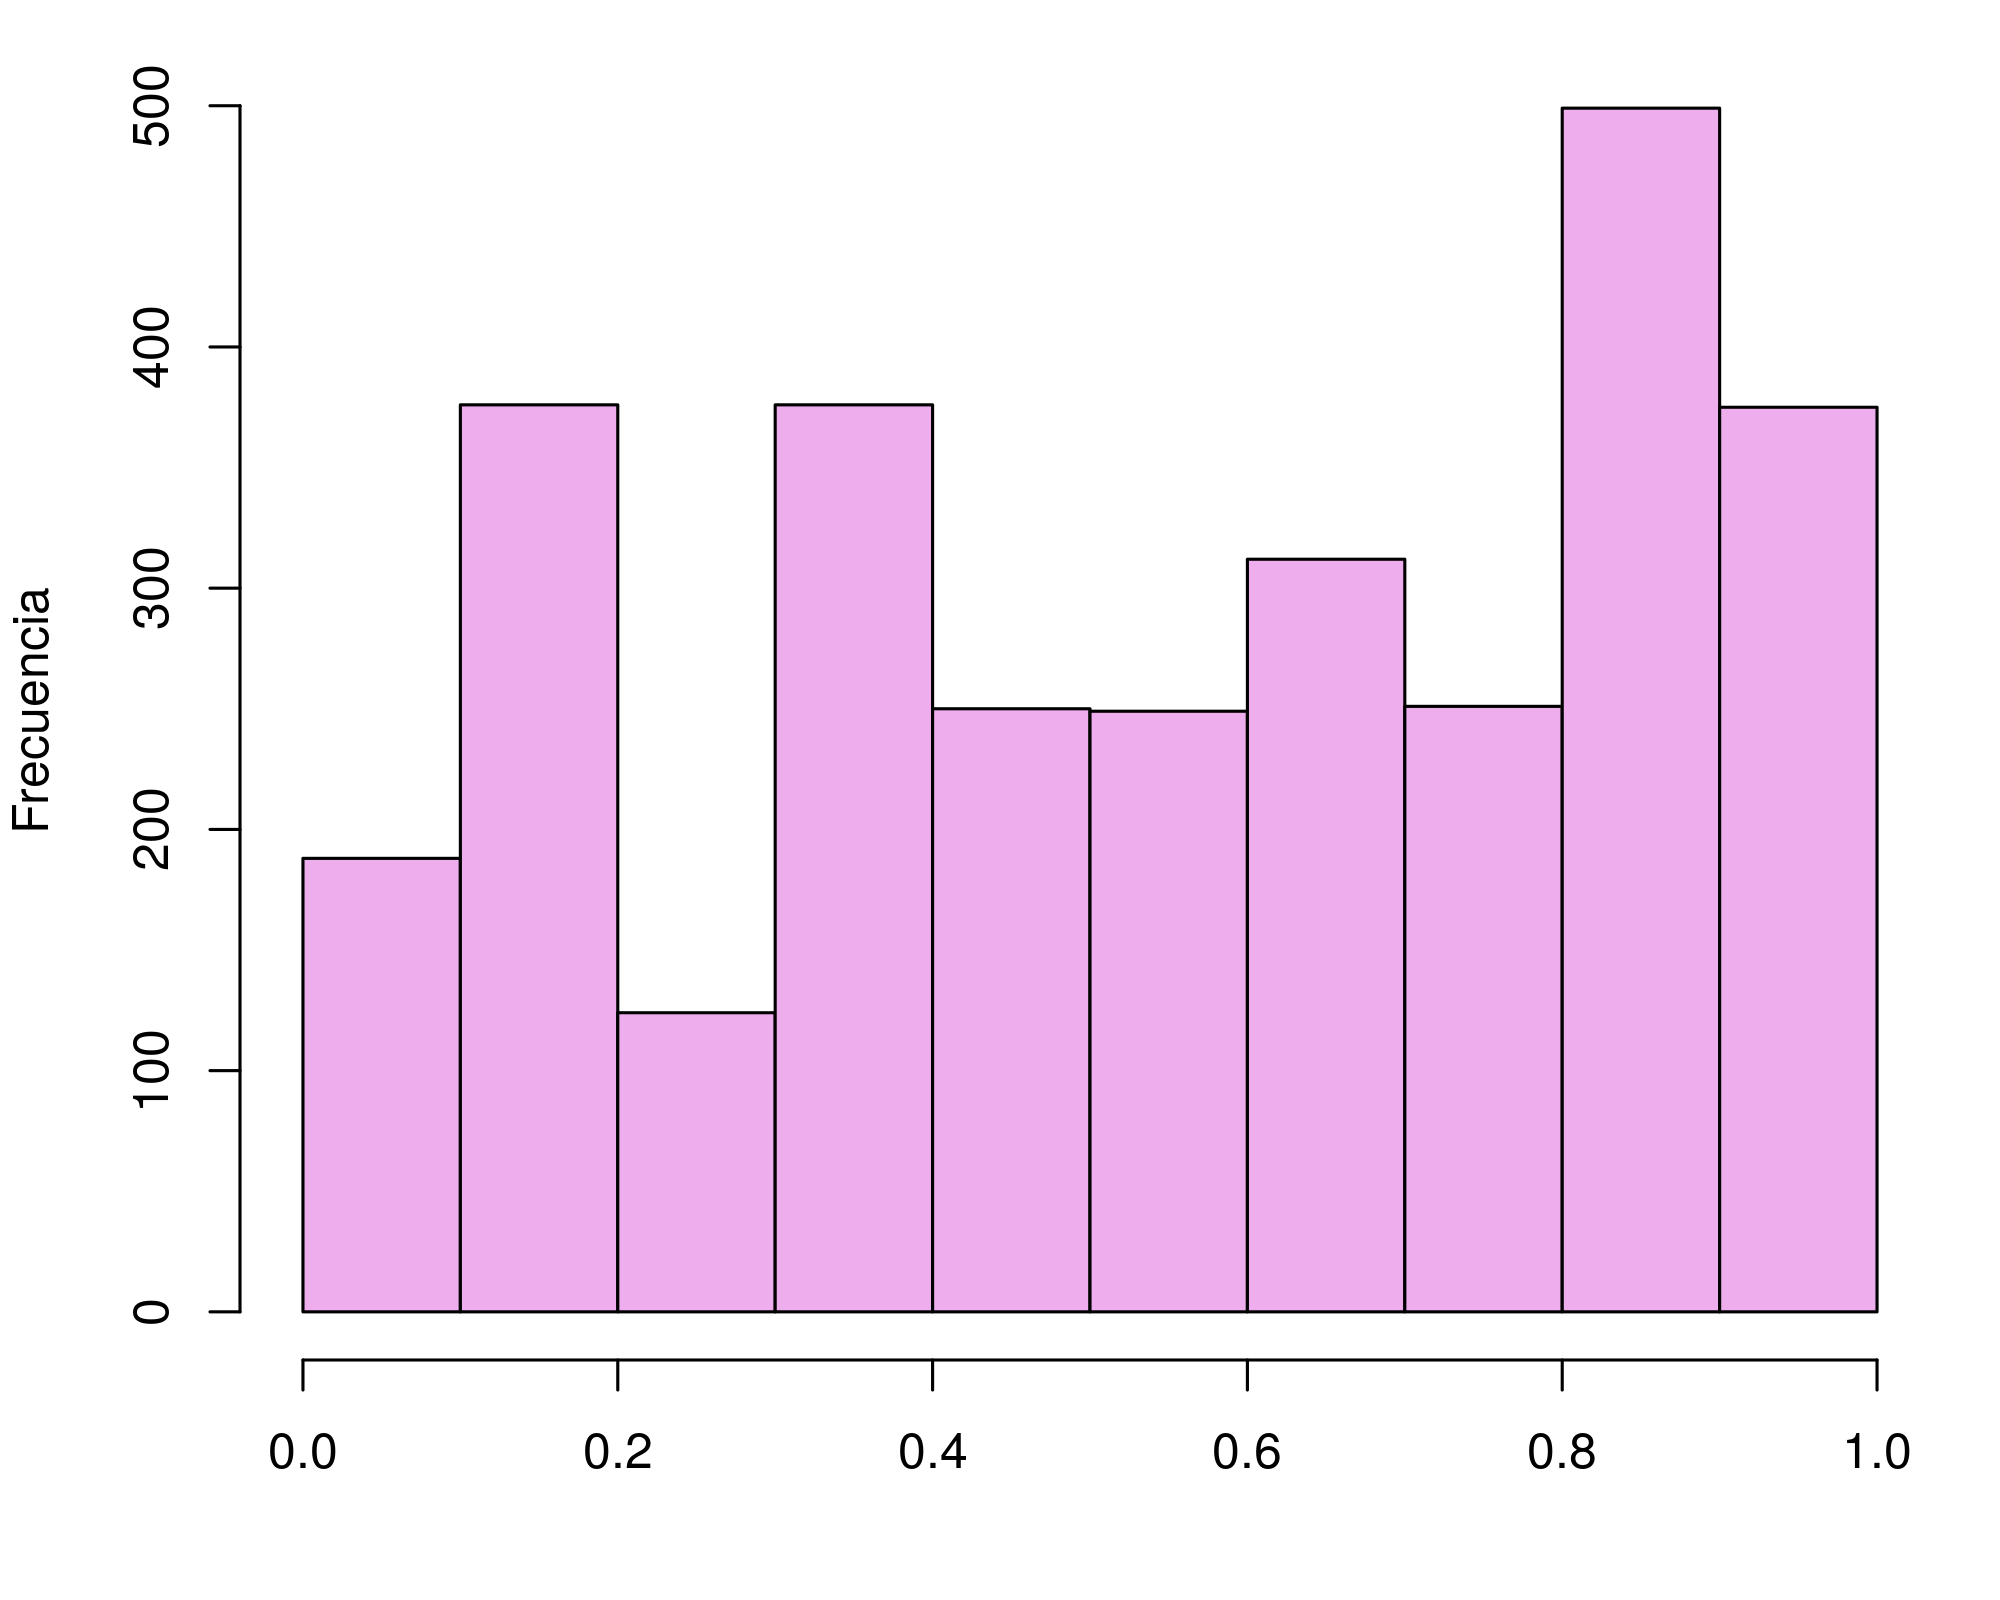
\includegraphics[scale=0.34]{hist_1117-11-43-97.png}
			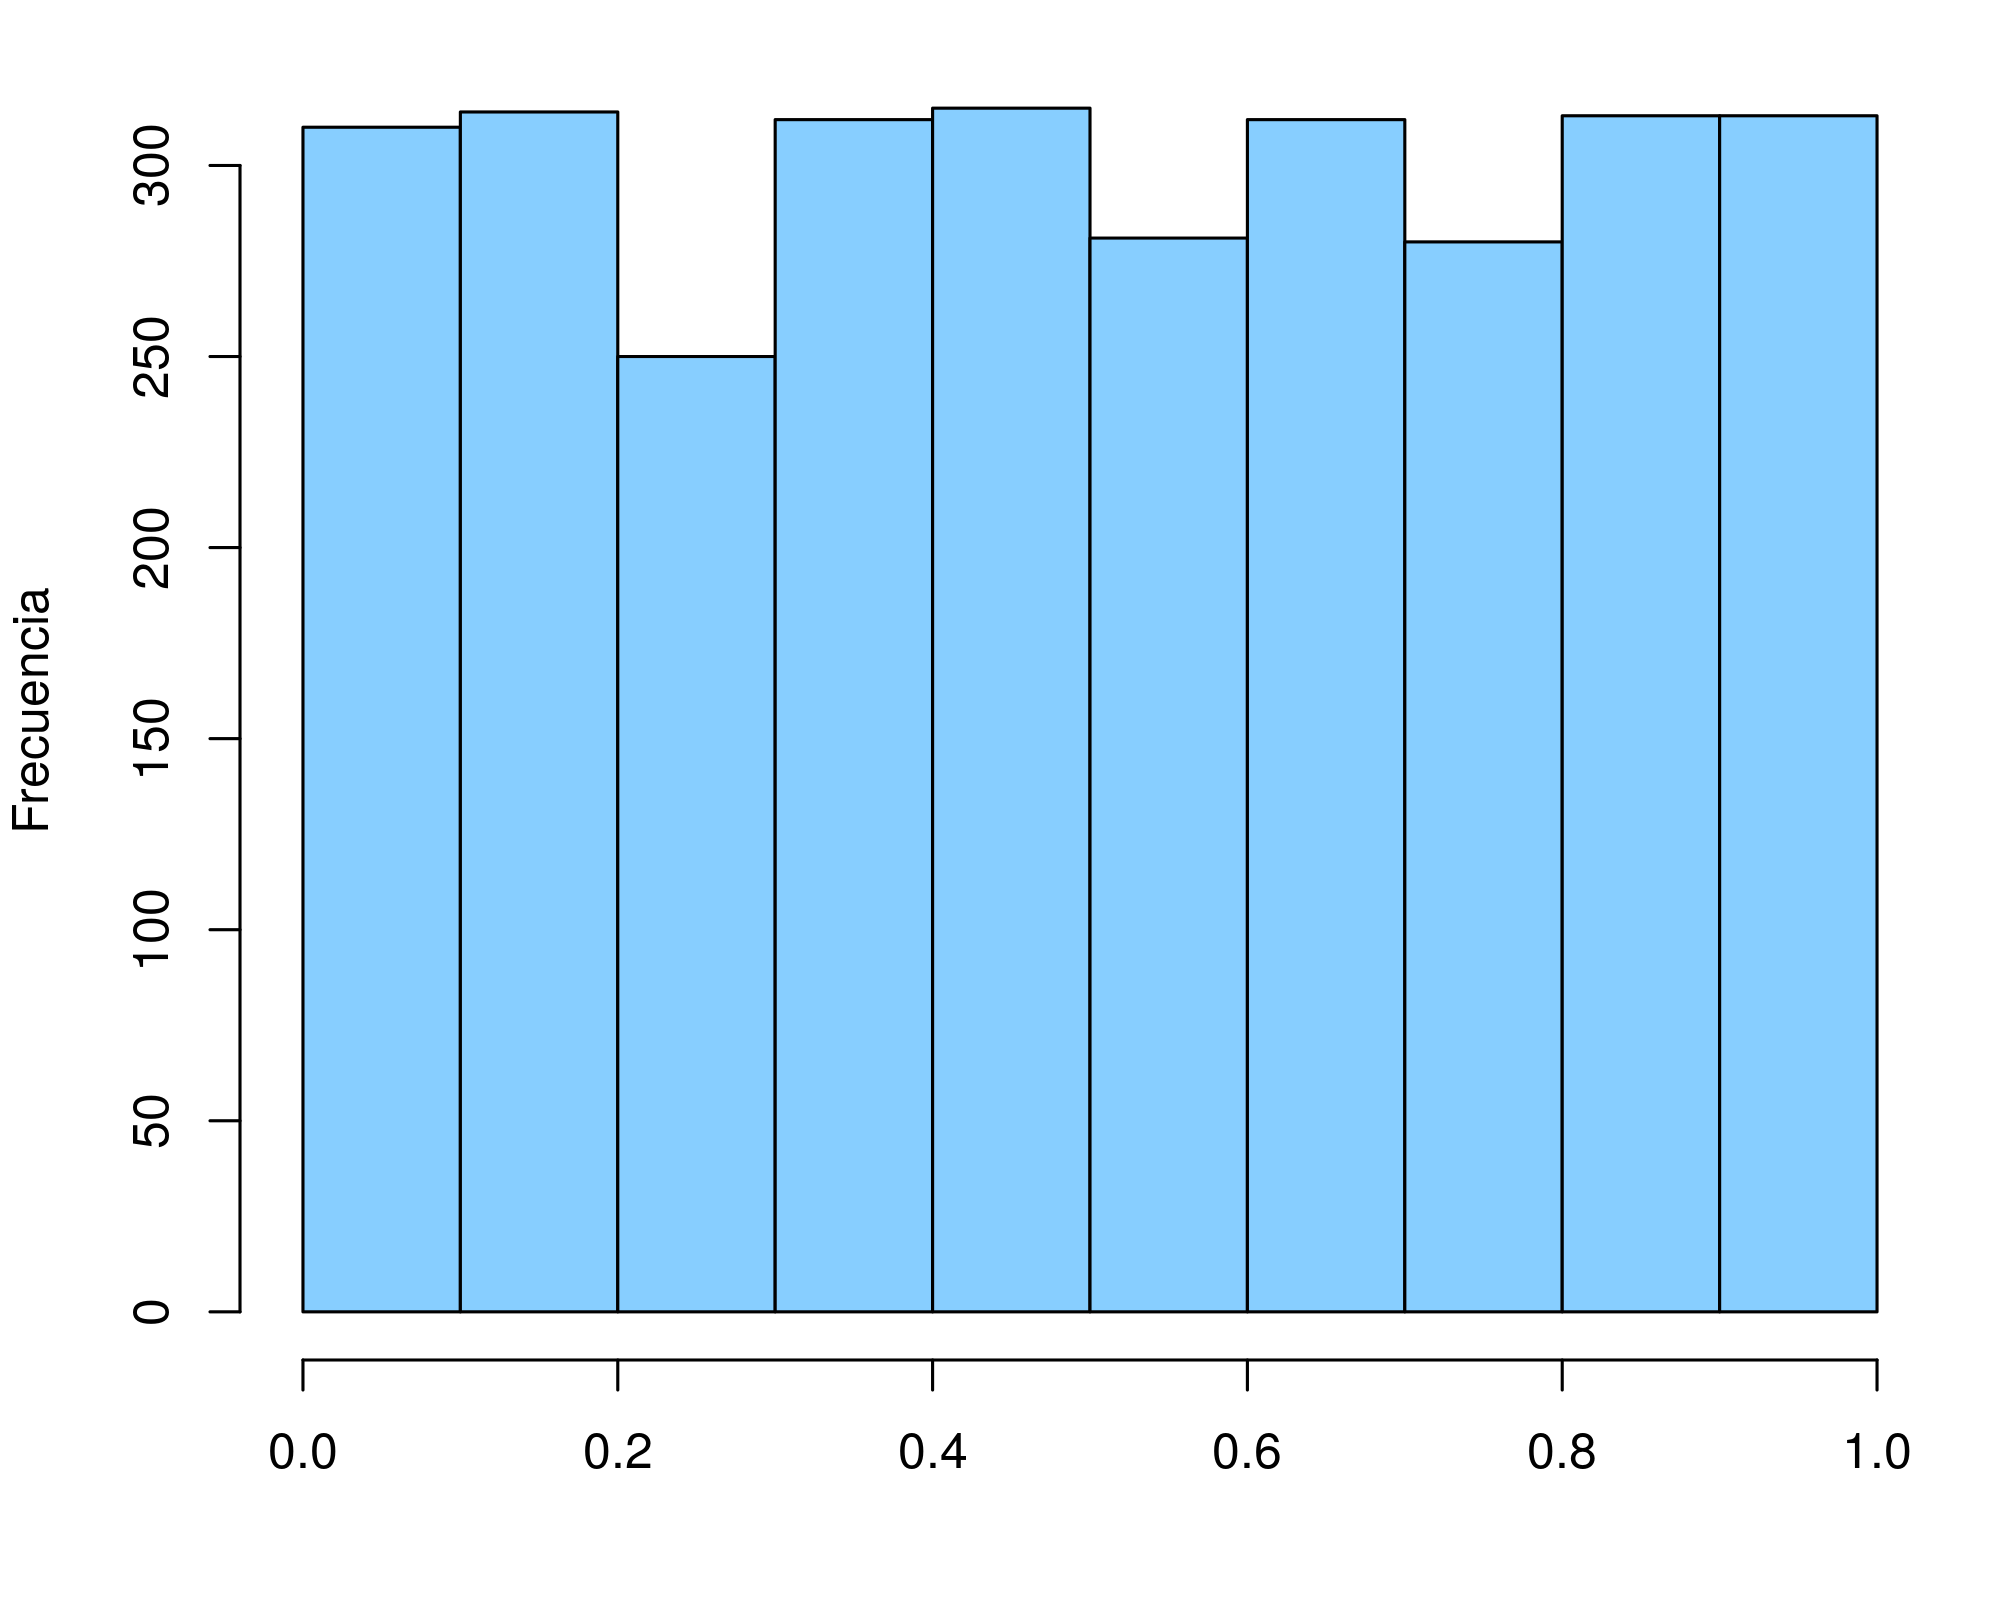
\includegraphics[scale=0.34]{hist_1117-59-43-97.png}
			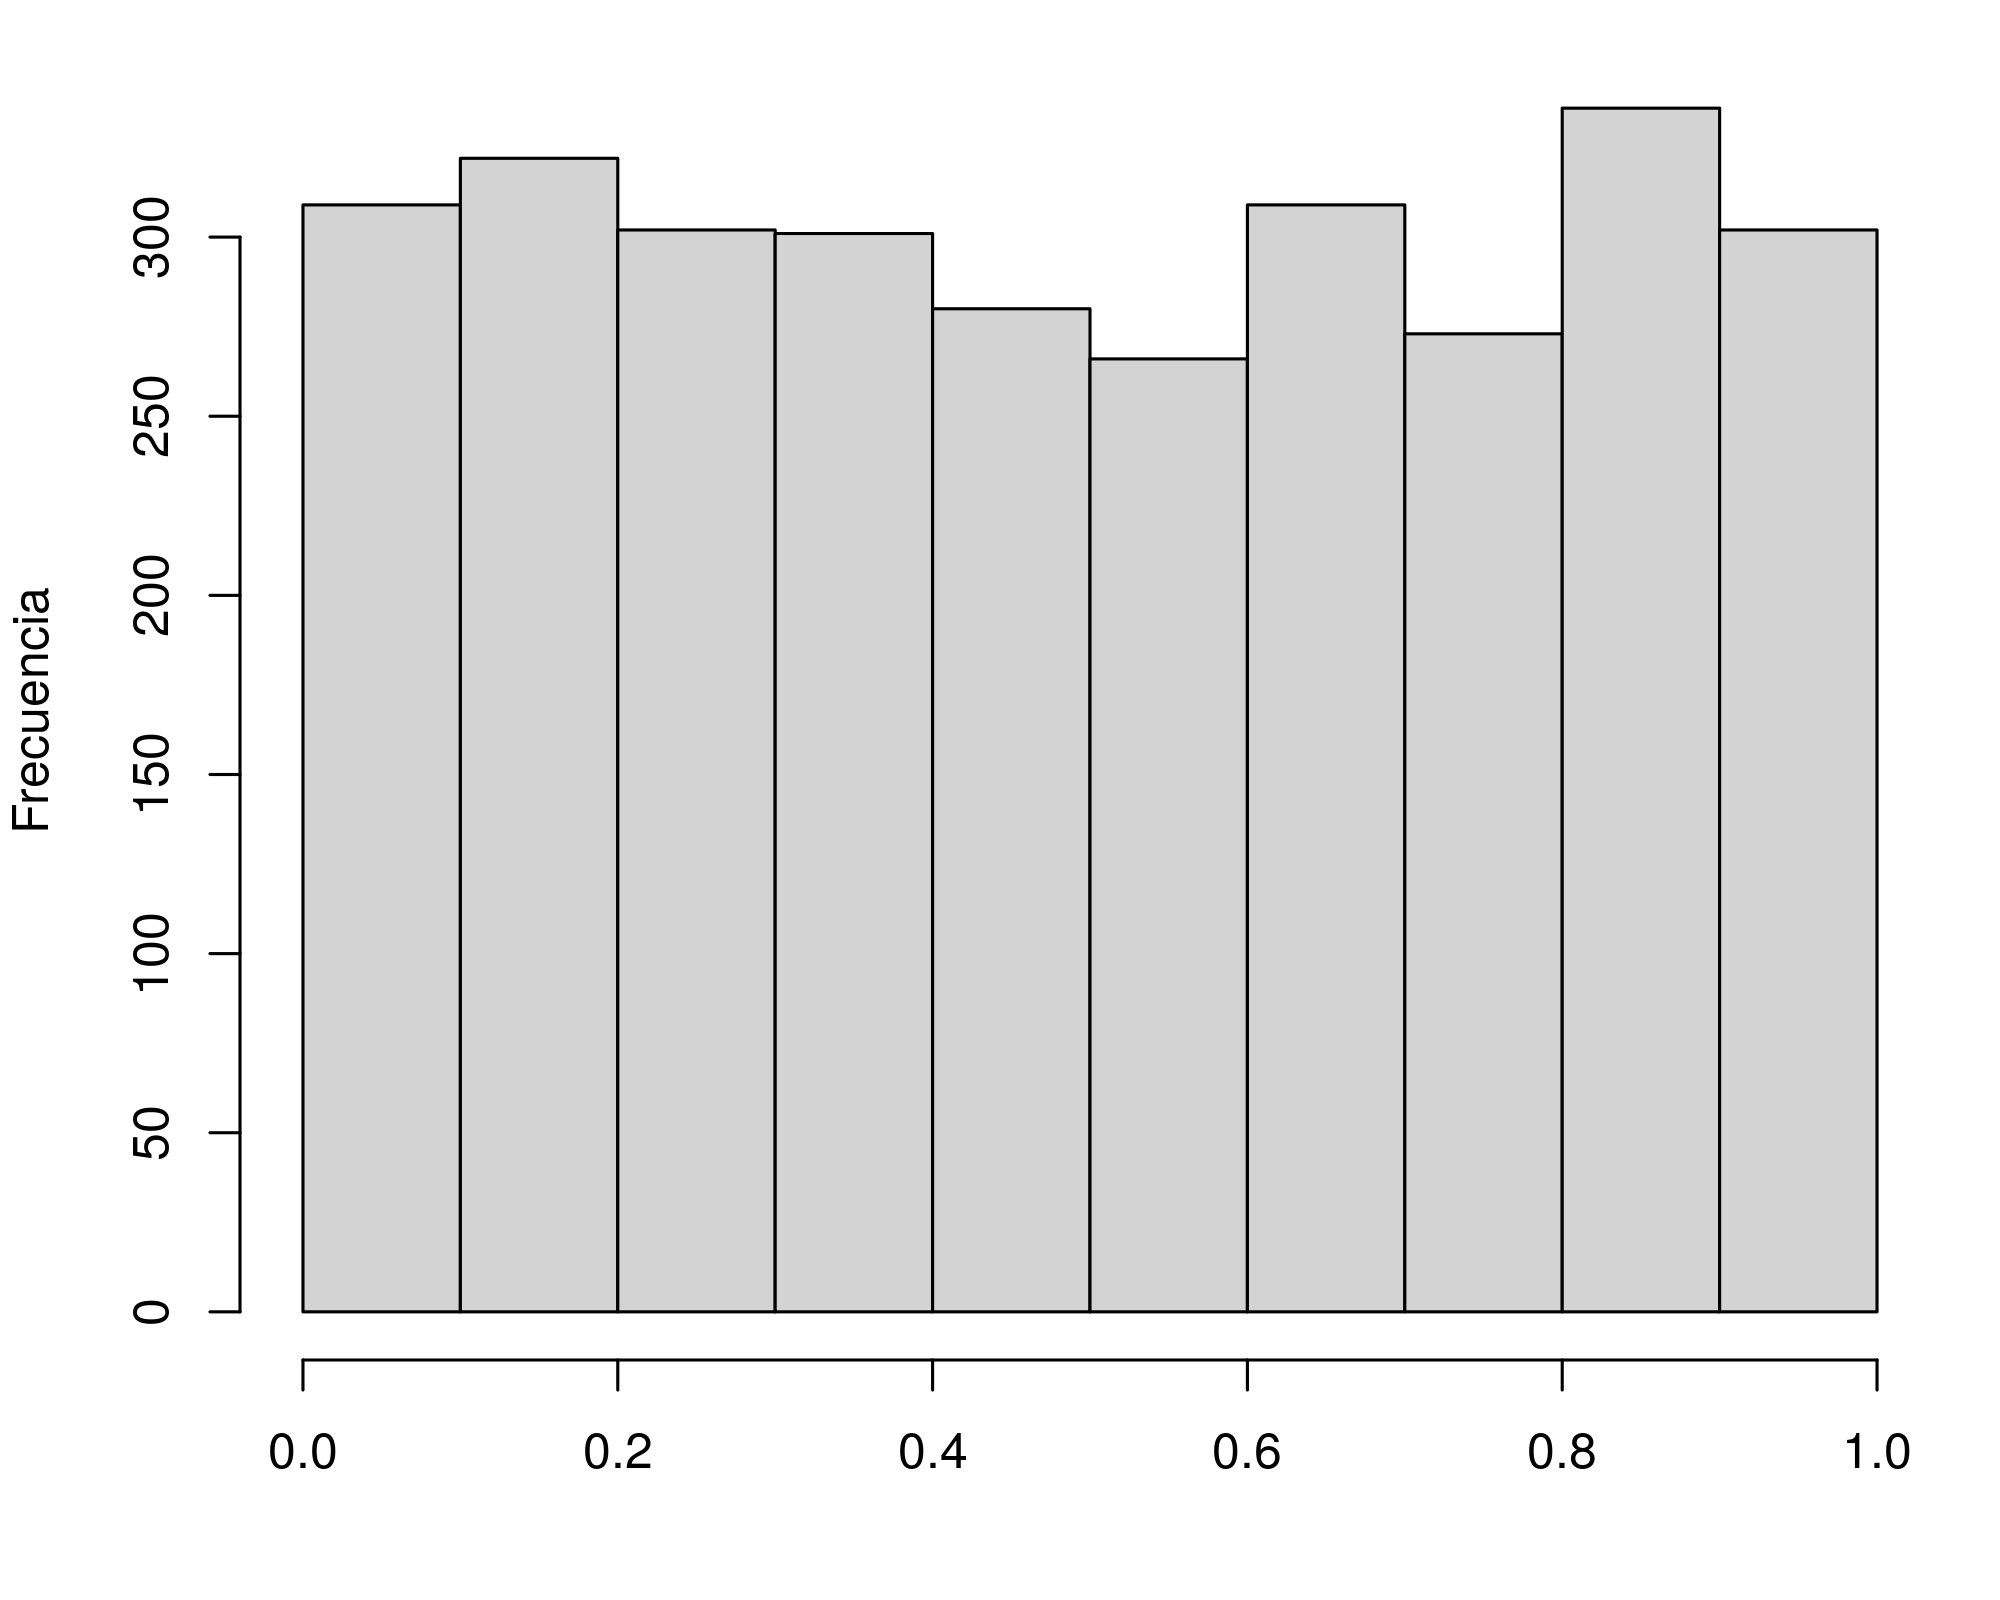
\includegraphics[scale=0.34]{hist_1117-613-919-857.png}
			\caption{$X_0 = 1117$.}
			\label{semilla1117}
		\end{subfigure}
		\caption{Distribución de la secuencia generada con las distintas configuraciones de parámetros. En rosa la generación con $a=11, c= 43$ y $m=97$; en azul con $a=59$, $c= 43$ y $m=97$ y, en gris con $a=613$, $c= 919$ y $m=857$.}
		\label{varia_semilla}
	\end{figure}

	El diagrama caja-bigote de la figura \ref{bigotes_semilla} muestra la variación en las secuencias generadas con la configuración $a=613$, $c= 919$ y $m=857$, cambiando el valor de la semilla. Claramente se observa que la variación entre los resultados es minúscula. Sin embargo, para comprobar estadísticamente si el valor de la semilla tiene un efecto considerable en la secuencia o no, se usa la prueba de {\em Kruskal-Wallis} \cite{kruskal_test} ya que se sabe que los datos no cumplen con la condición de normalidad que un análisis ANOVA requiere. 
	
	\begin{figure}
		\centering
		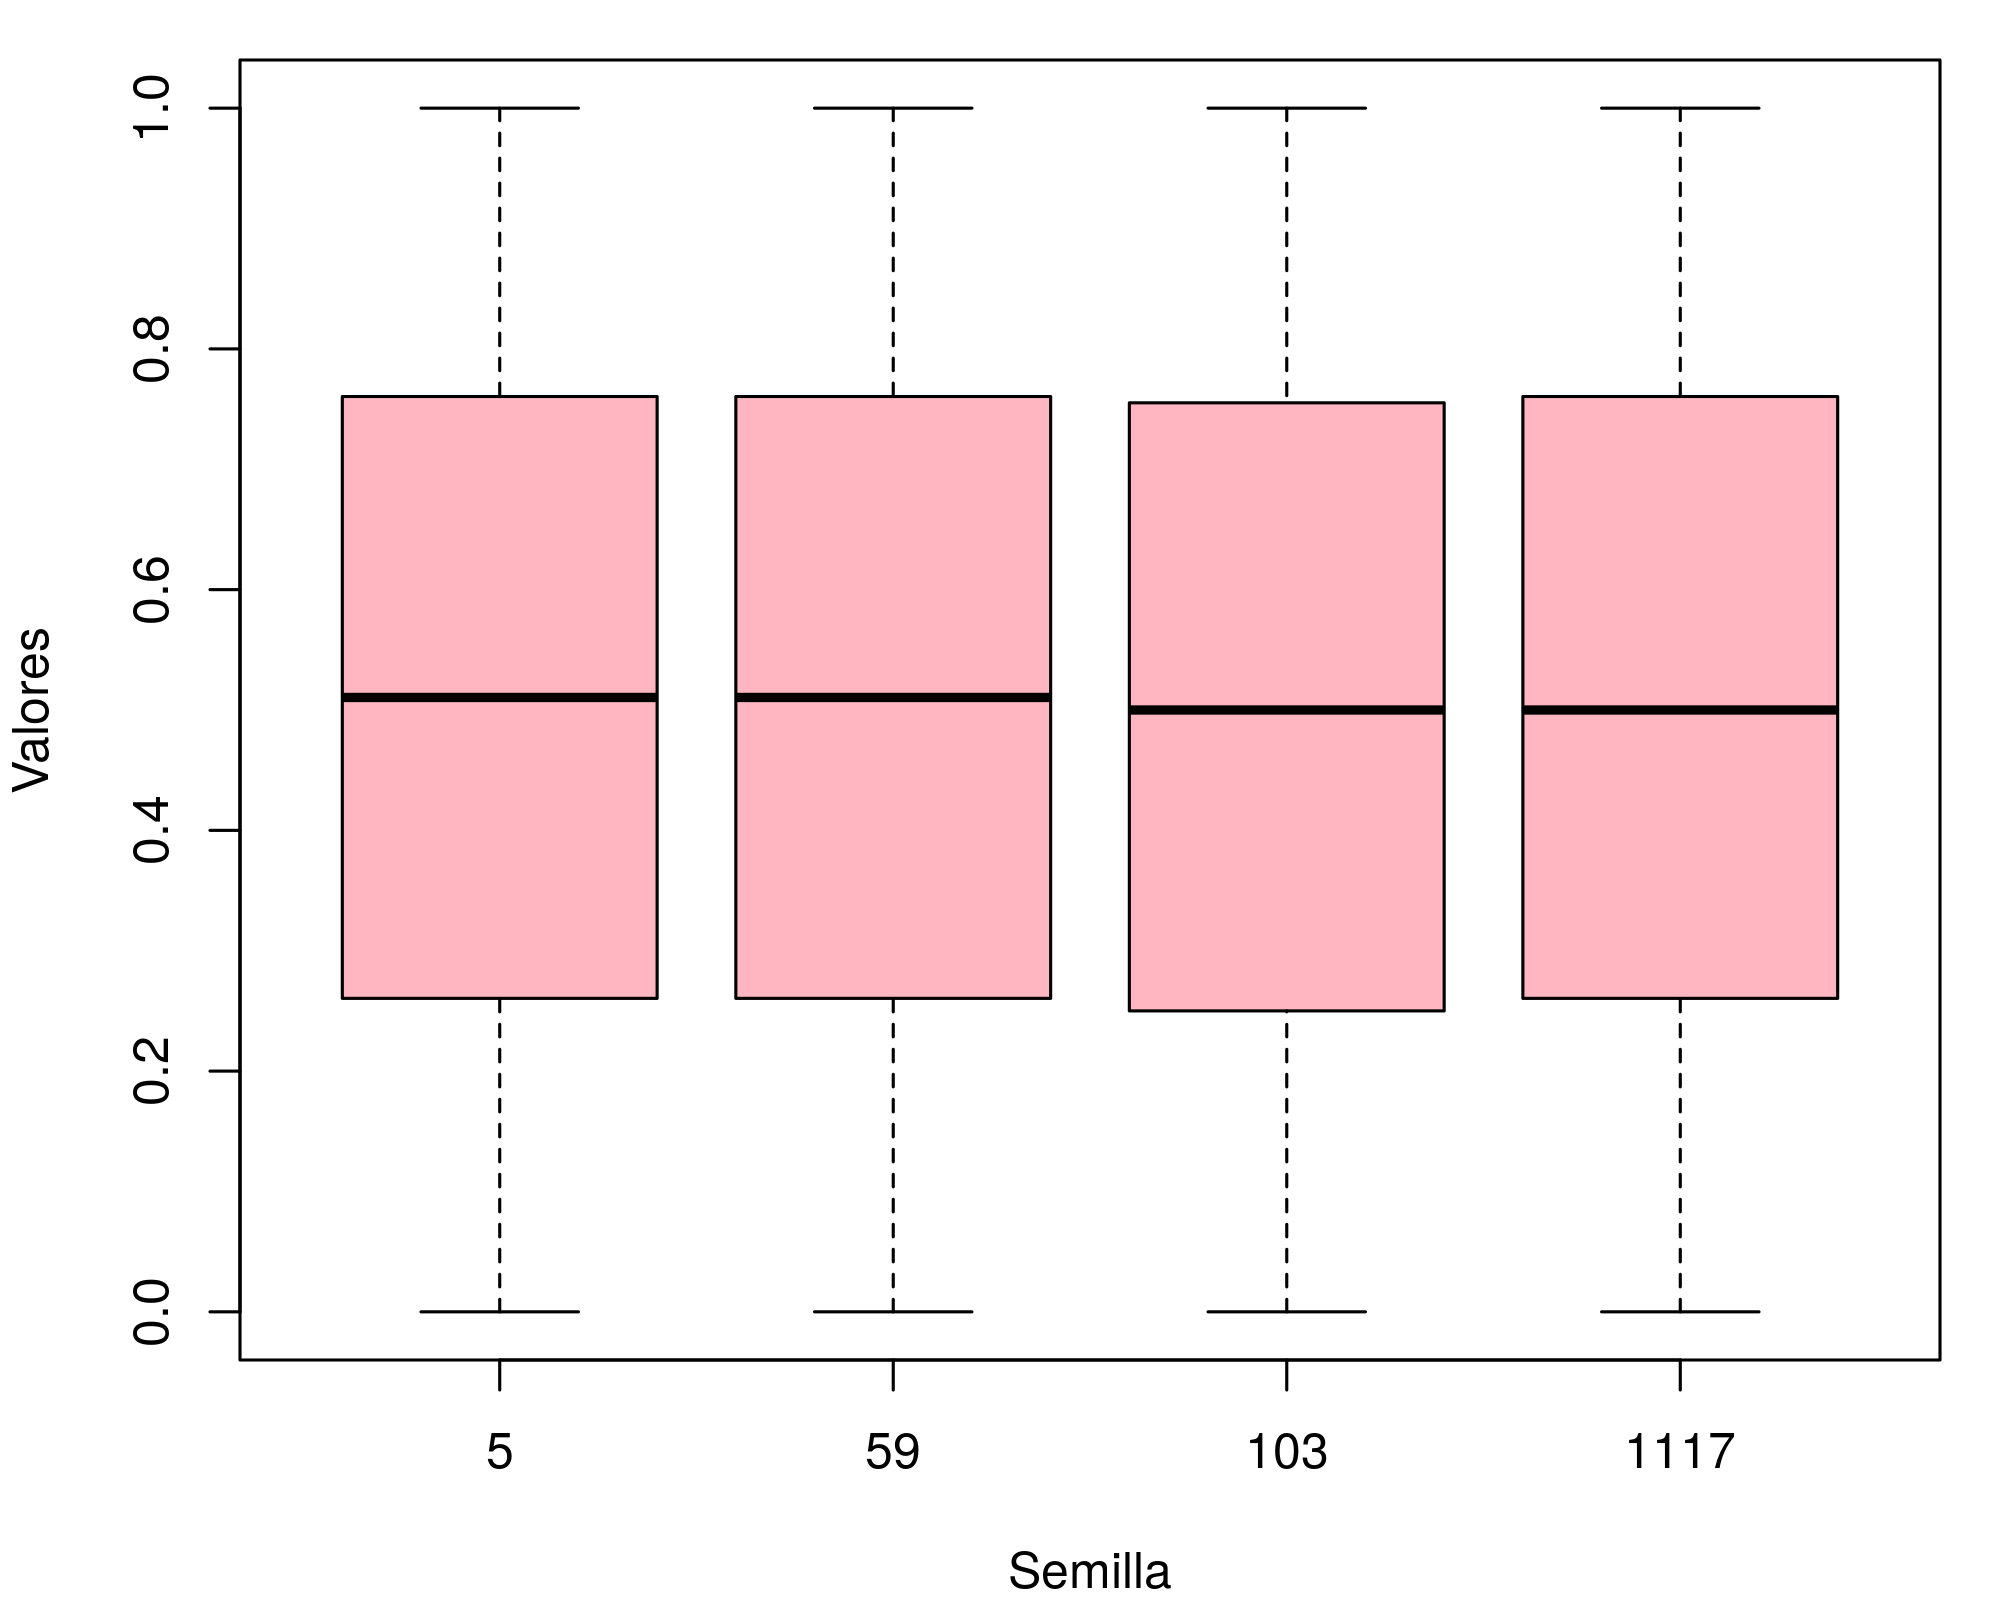
\includegraphics[scale=0.6]{var_semilla.png}
		\caption{Variación de las secuencias generadas usando $a=613$, $c= 919$ y $m=857$, cambiando el valor de la semilla.}
		\label{bigotes_semilla}
	\end{figure}
	
	La prueba de {\em Kruskal-Wallis} considera como hipótesis nula que {\em todas las muestras provienen de una misma distribución}. El resultado de aplicar la prueba a los resultados de la configuración $a=613$, $c= 919$ y $m=857$ se muestra a continuación.
	\begin{verbatim}
	Kruskal-Wallis rank sum test

	data:  valores by semilla
	Kruskal-Wallis chi-squared = 0.61394, df = 3, p-value = 0.8932
	\end{verbatim}
	 
	El $p$-valor obtenido nos permite concluir que la variación en la semilla no tiene un efecto significativo en la secuencia generada. Al aplicar la prueba para la configuración $a=59$, $c= 43$ y $m=97$, se llega al mismo resultado. 
	
	
	\section{Método de Box-Muller}
	
	El método Box-Muller genera pares de números aleatorios con distribución normal de media cero y desviación estándar igual a uno. Para la generación utiliza como fuente números aleatorios uniformemente distribuidos.
	
	Siendo $u_1$ y $u_2$ dos números independientes obtenidos de una distribución uniforme, la generación mediante el método se realiza con las ecuaciones (\ref{z0}) y (\ref{z1}).
	\begin{eqnarray}
	z_0 &=& \left( \sqrt{-2 \ln u_1} \cdot \cos(2\pi u_2)\right) \sigma + \mu , \label{z0} \\
	z_1 &=& \left(  \sqrt{-2 \ln u_1} \cdot \sin(2\pi u_2) \right) \sigma + \mu . \label{z1}
	\end{eqnarray} 

	Un primer análisis estudia si usar sólo uno de estos valores genera diferencias en los datos. La figura \ref{uno_ambos} muestra las diferentes distribuciones que se generan con el método al usar sólo uno de los valores y ambos. Las tres distribuciones pasan la prueba de normalidad de {\em Shapiro} con un $p$-valor de 0.5854184, 0.1078563, 0.2750796, usando sólo $z_0$, $z_1$ y ambos, respectivamente.
	
	\begin{figure}
		\begin{subfigure}{\textwidth}
			\centering
			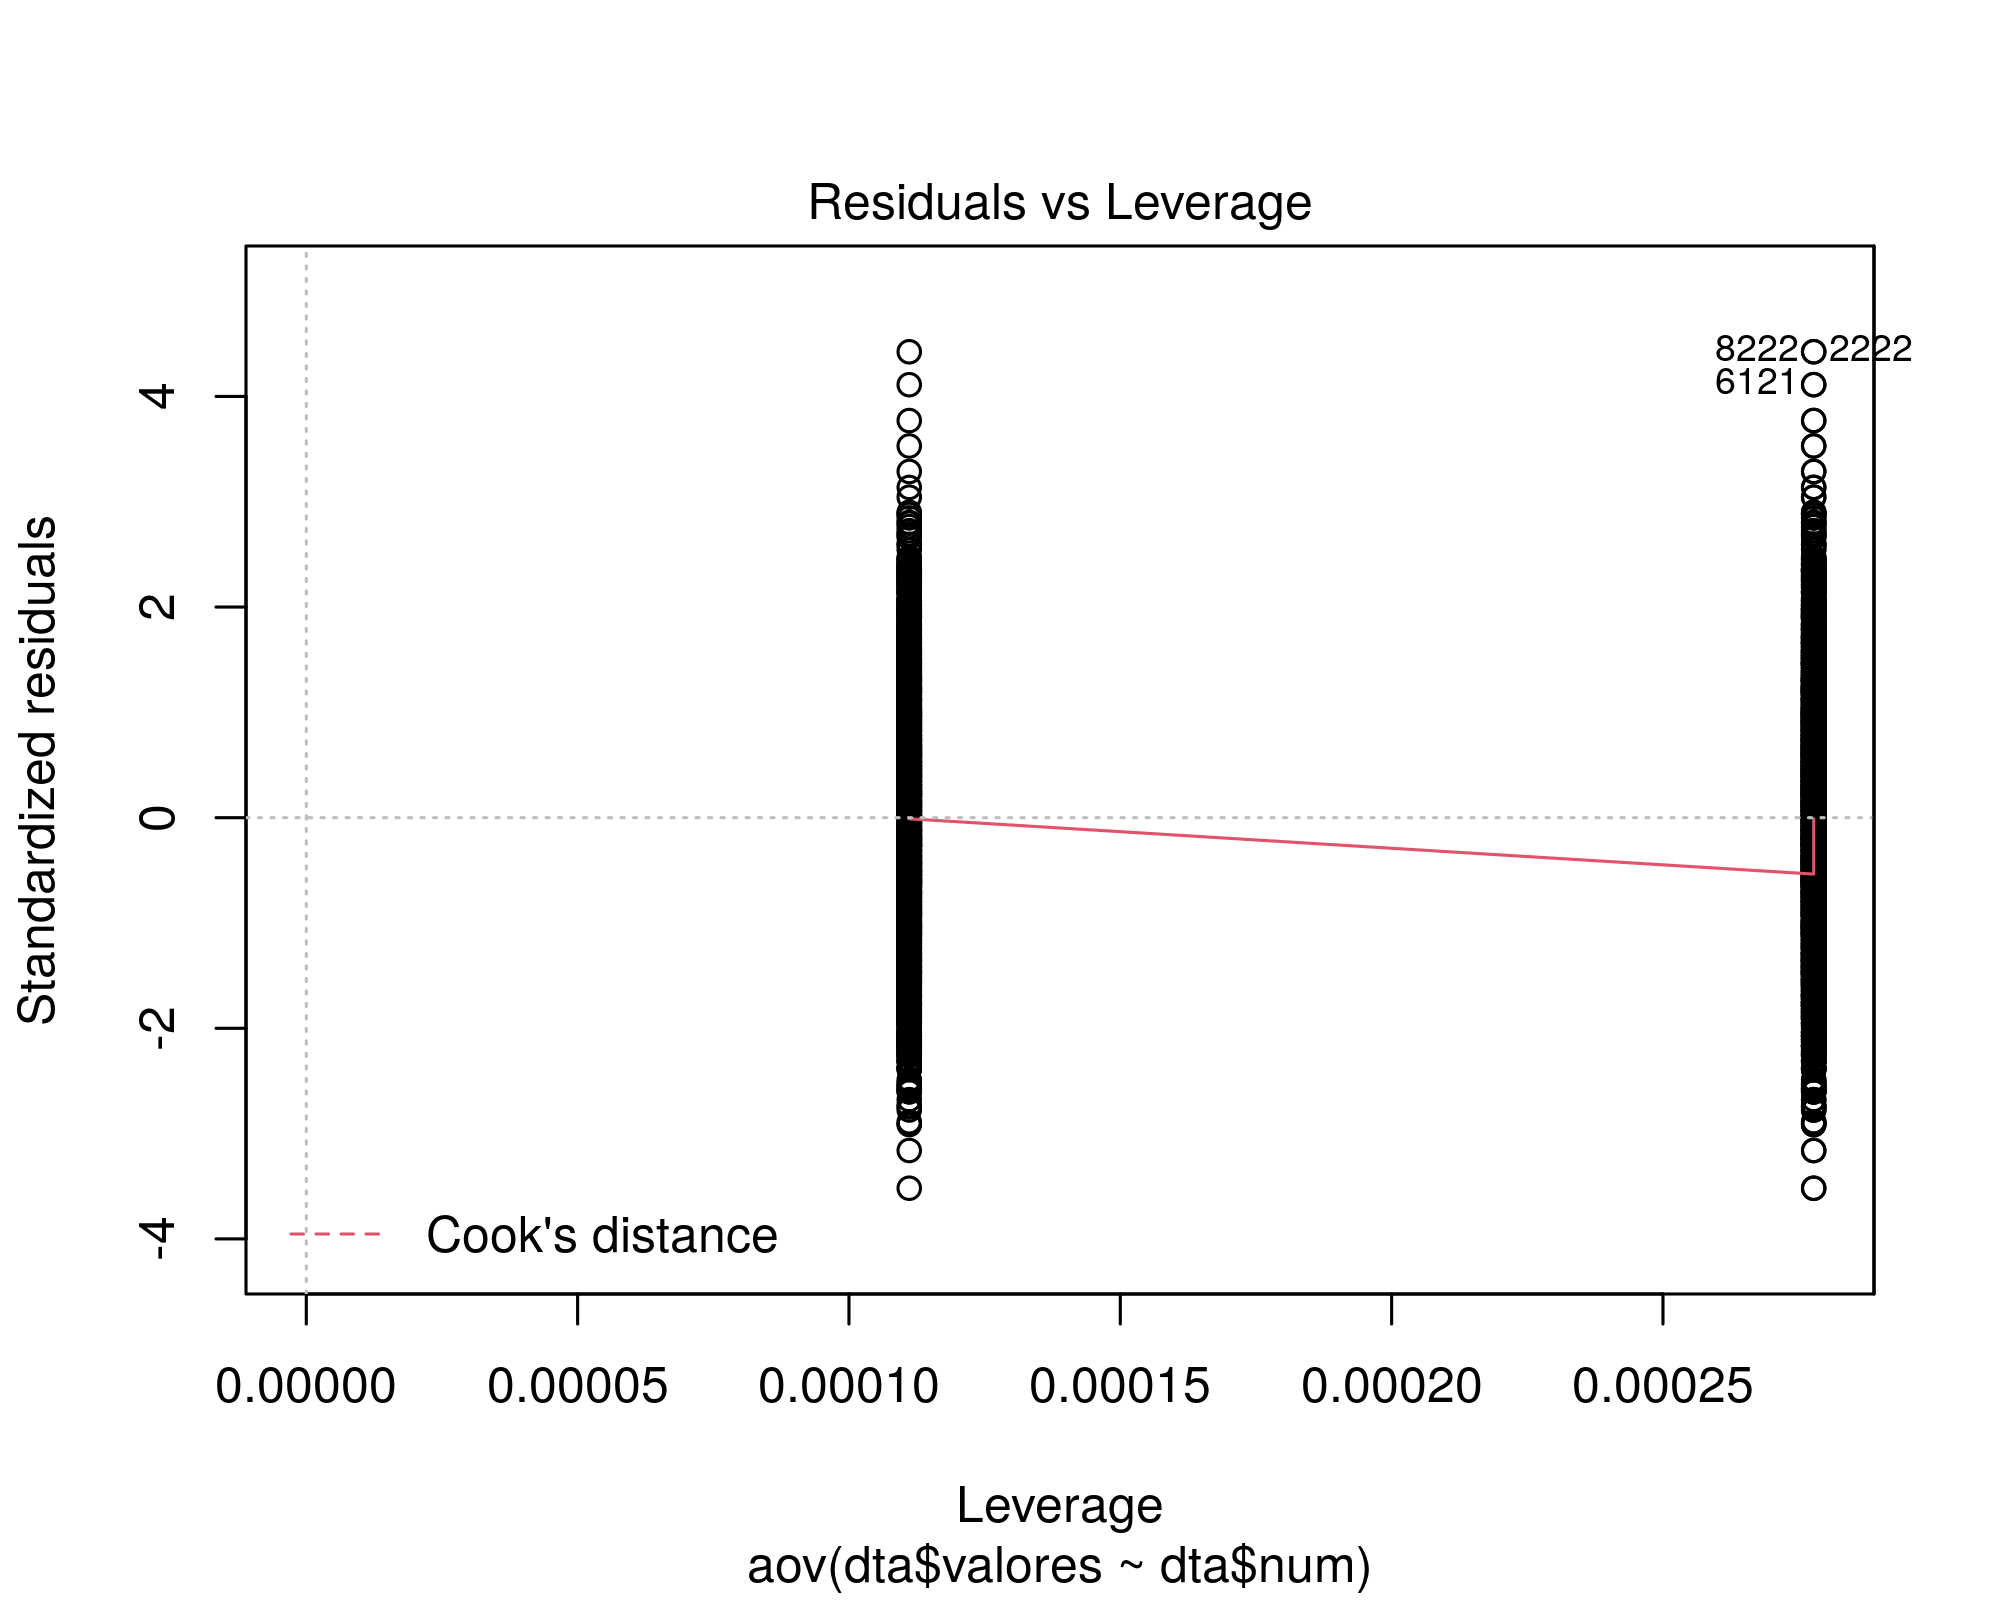
\includegraphics[scale=0.45]{normalz0.png}
			\caption{Sólo $z_0$.}
		\end{subfigure}
		\begin{subfigure}{\textwidth}
			\centering
			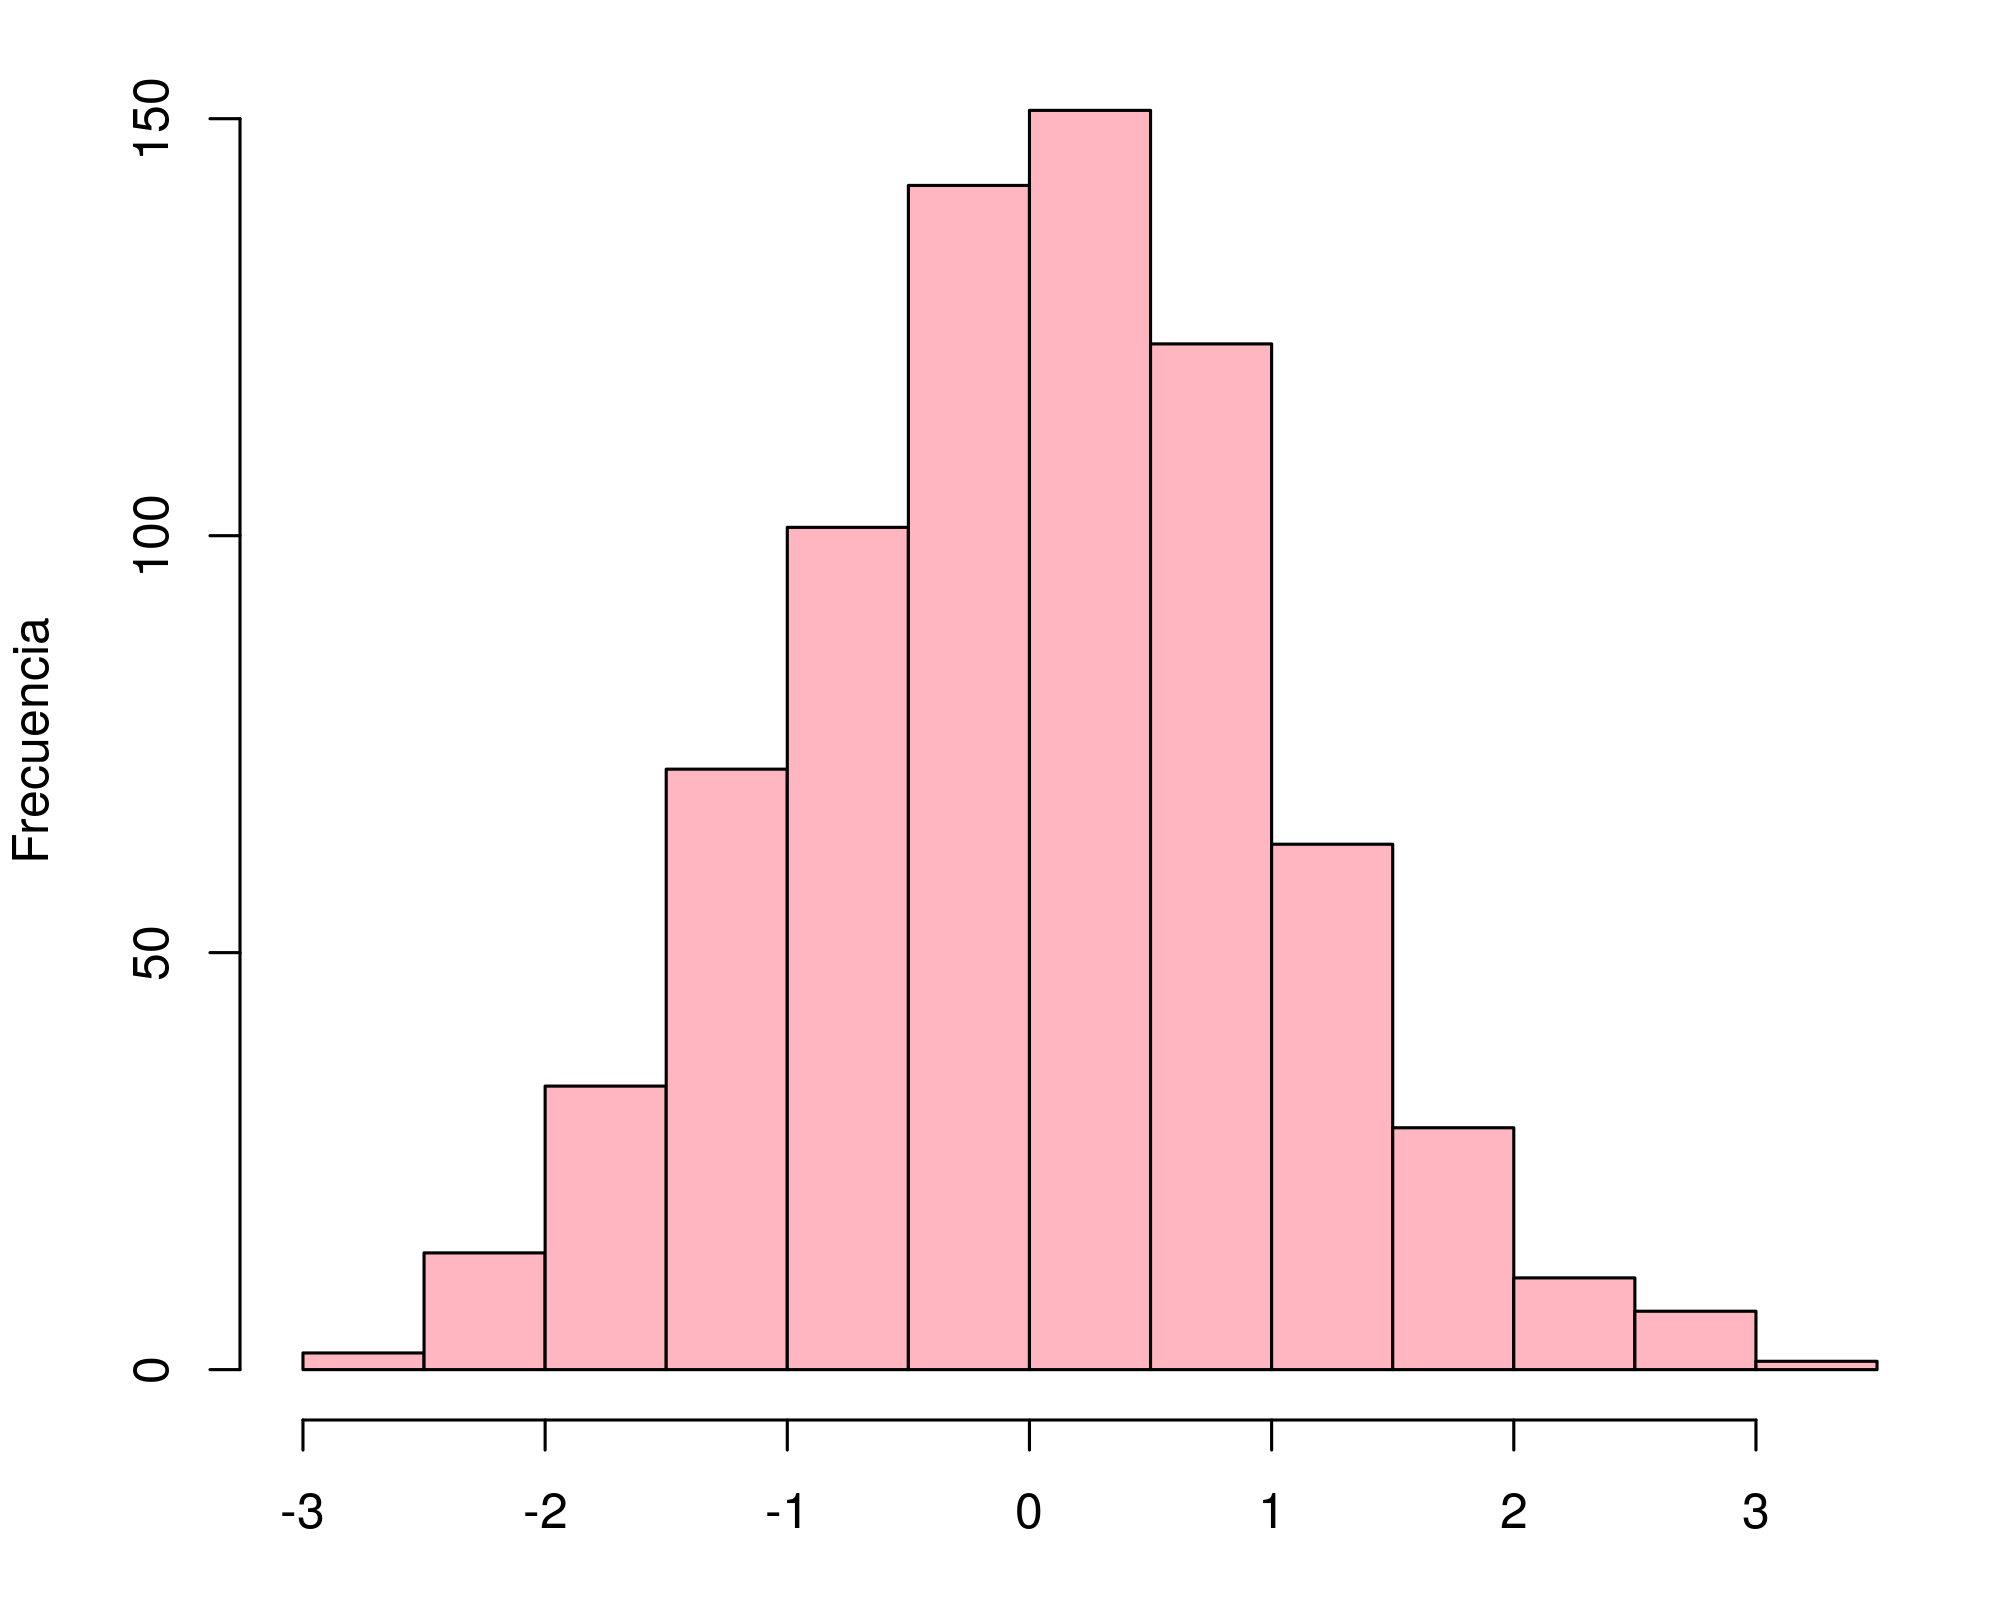
\includegraphics[scale=0.45]{normalz1.png}
			\caption{Sólo $z_1$.}
		\end{subfigure}
		\begin{subfigure}{\textwidth}
			\centering
			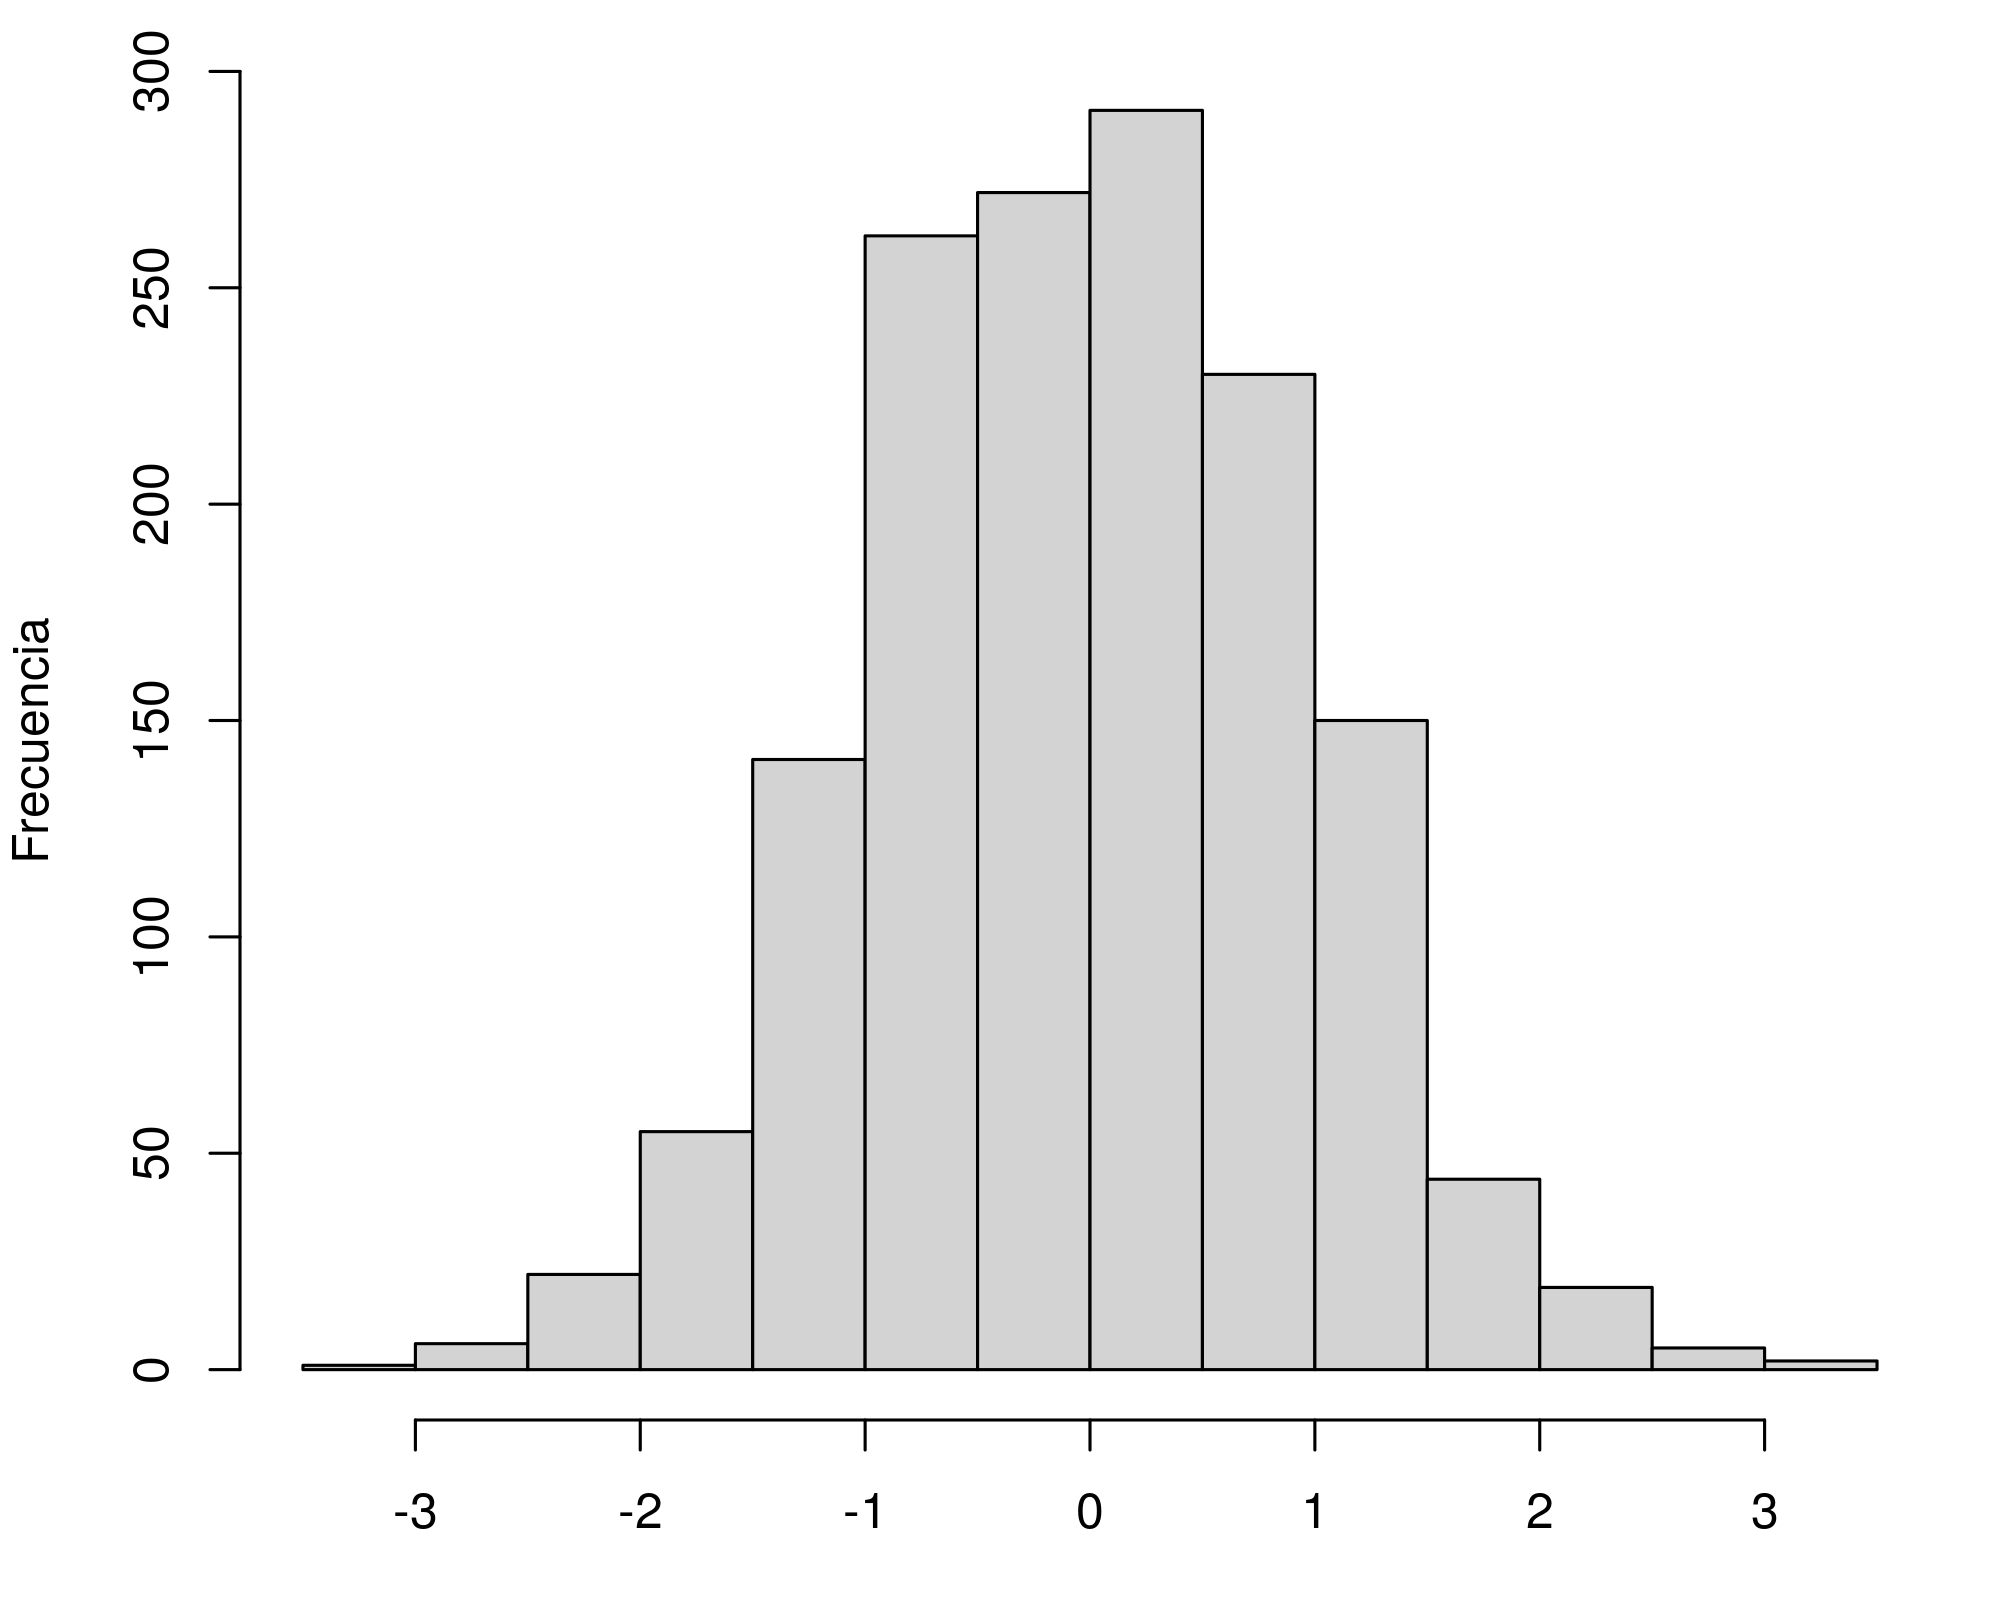
\includegraphics[scale=0.45]{normalambos.png}
			\caption{Ambos.}
		\end{subfigure}
	\caption{Distribuciones generadas por el método usando sólo $z_0$, $z_1$ o ambos valores.}
	\label{uno_ambos}
	\end{figure}

	En la sección anterior se estudió un método para generar números uniformes, así que se hace una combinación con el método de Box-Muller. En lugar de usar la función \texttt{runif} de \textsc{R} para obtener los valores $u_1$ y $u_2$, se usa la función \texttt{uniforme.R} que es un generador lineal congruencial.
	
	El análisis previo del generador lineal congruencial, permitió identificar dos configuraciones que dan ``buenas'' y ``malas'' secuencias de números uniformemente distribuidos. La pregunta ahora es, si se usan buenos y malos valores de $u_1$ y $u_2$, ¿qué pasa con la calidad de la secuencia que se genera? ¿pierde la normalidad?.
	
	El experimento que se plantea para realizar este estudio es el siguiente: se crea la secuencia de $n=1000$ números mediante generador lineal congruencial con una de las configuraciones previas y se crea la secuencia con el método de Box-Muller tomando $u_1$ y $u_2$ aleatorios de la secuencia generada en el paso anterior. Esta ultima también de tamaño $n=1000$. Se realizan diez réplicas del experimento, para cada una de ellas se verifica la normalidad con la prueba de {\em Shapiro}.
	
	Se sabe que la configuración $x_0 = 1117$, $a=3$, $c=5$ y $m=7$ no da una secuencia mala de números ya que sólo tiene seis valores diferentes, entre los cuales se encuentra el valor cero. Esto representa un problema para el método de Box-Muller porque para calcular $z_0$ y $z_1$ se usa la función logaritmo que no está definida para ese valor. 
	
	La figura \ref{normal_malo} muestra la distribución obtenida con el método de Box-Muller usando el generador lineal congruencial con la configuración de parámetros $x_0 = 1117$, $a=3$, $c=5$ y $m=7$ en contraste con la distribución generada a partir de la función \texttt{rnorm}. Se puede observar que una mala calidad de valores $u_1$ y $u_2$ generan una mala calidad de valores $z$.
	
	\begin{figure}
		\centering
		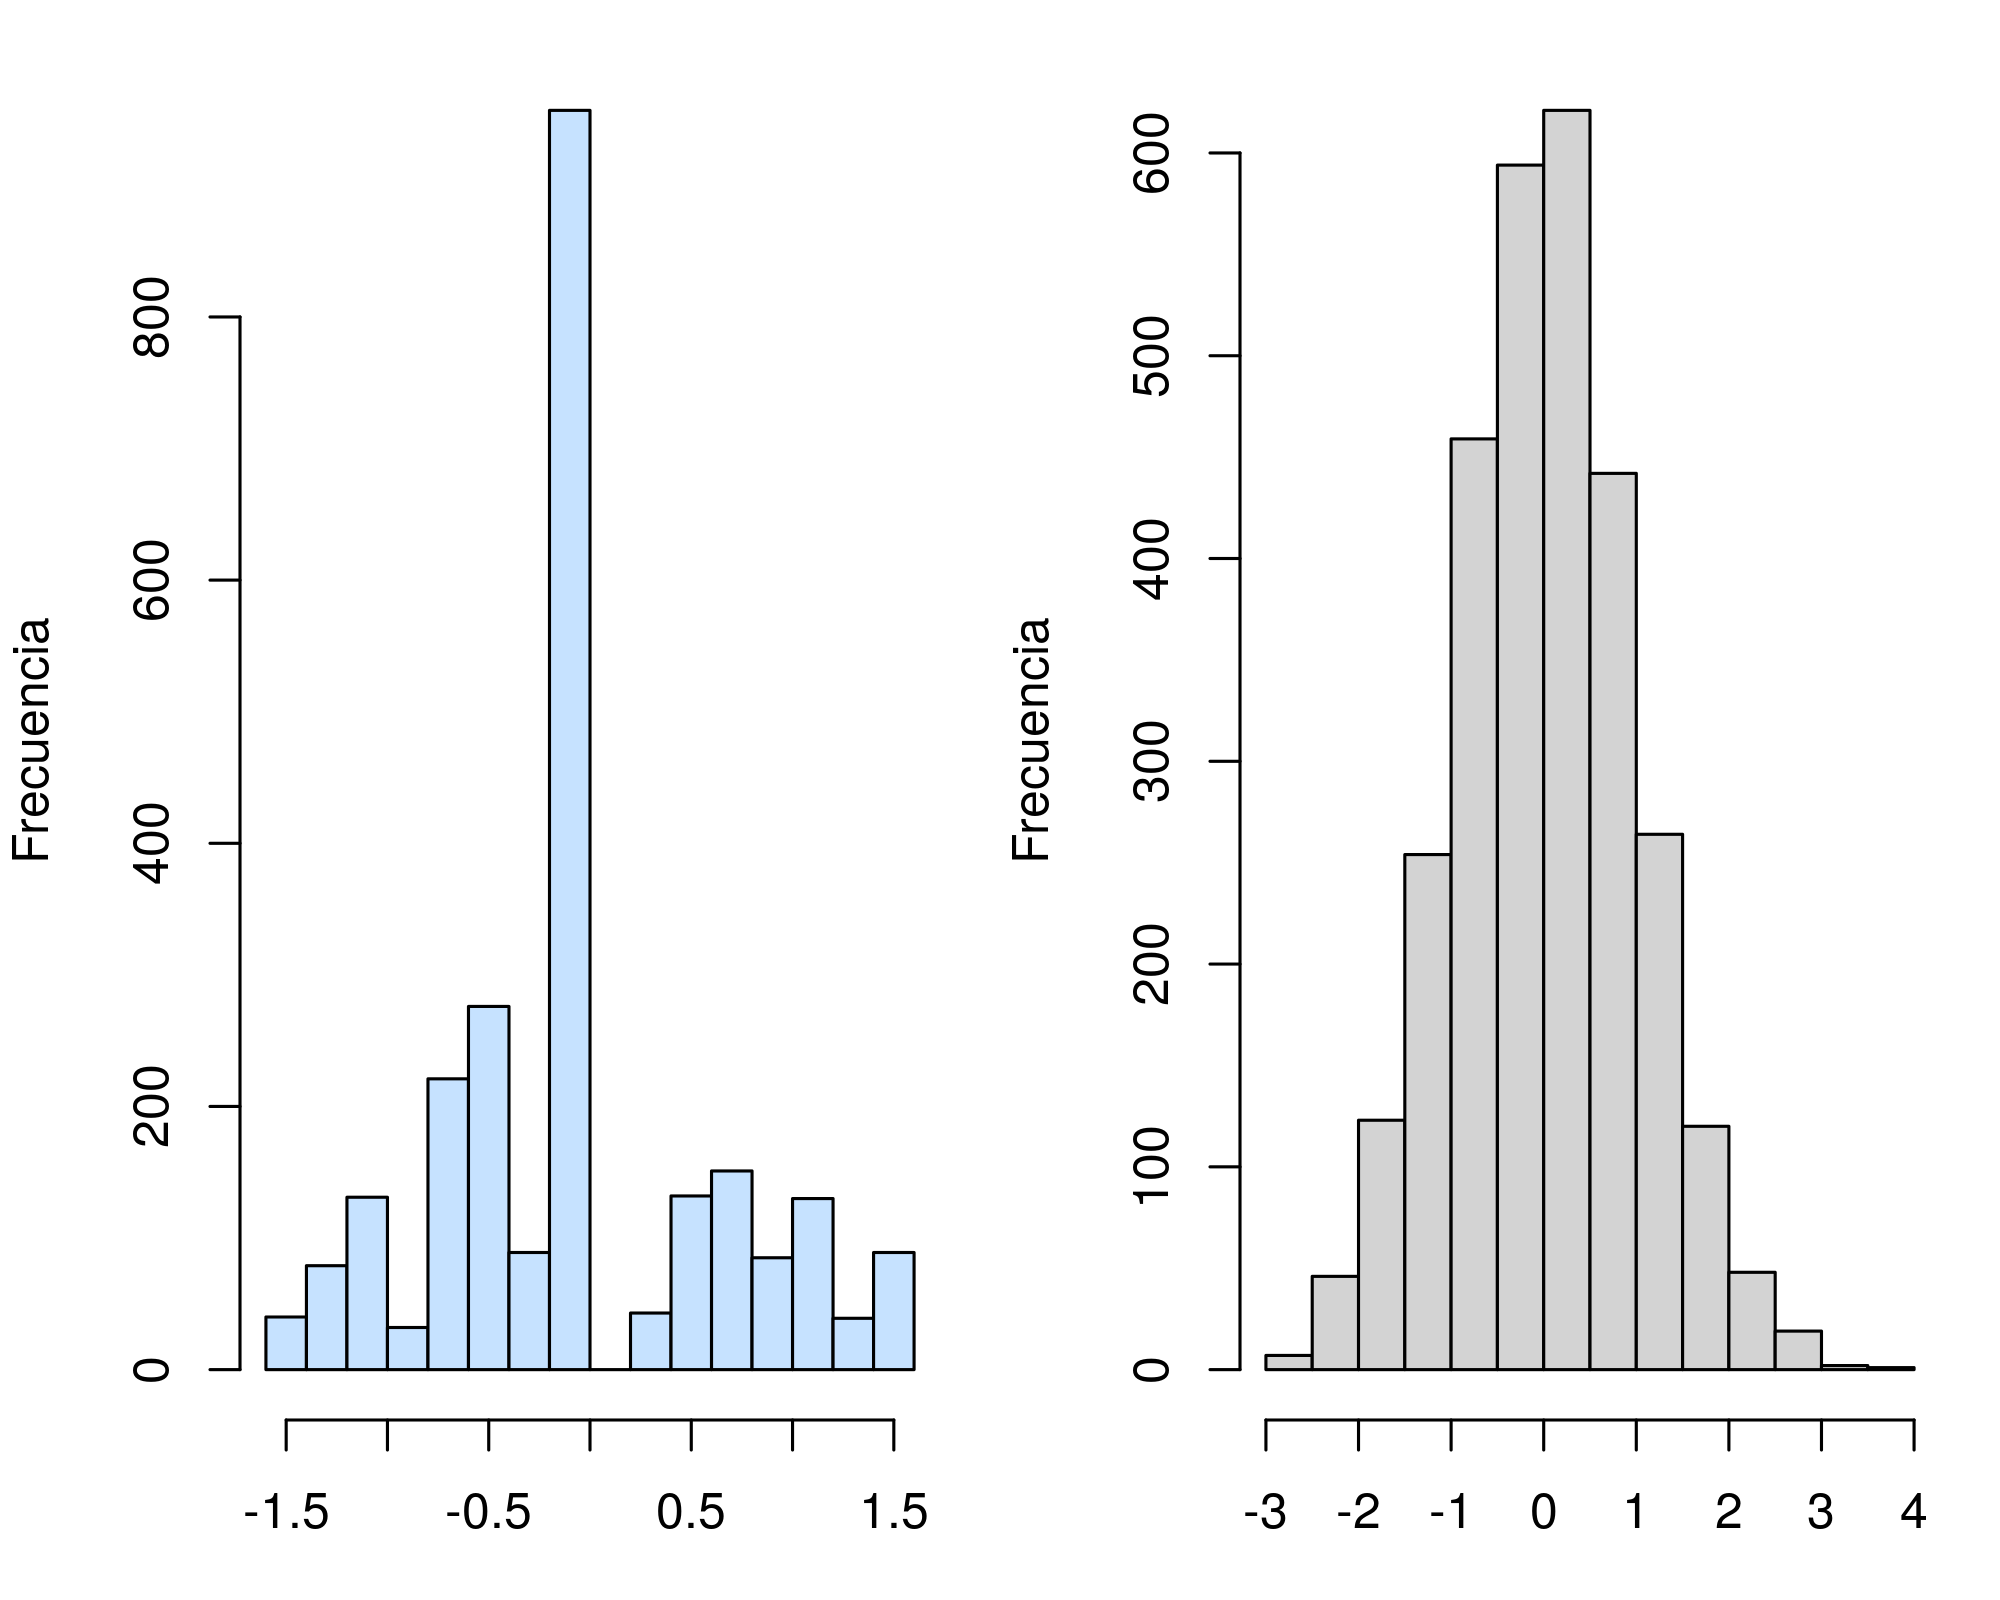
\includegraphics[width=0.6\textwidth]{normal_uniforme_malo.png}
		\caption{Distribución normal. En azul, la distribución generada por el método de Box-Muller usando el generador lineal congruencial con parámetros ``malos'' y en gris la distribución generada por \texttt{rnorm(n)}.}
		\label{normal_malo}
	\end{figure}

	Finalmente, la figura \ref{normal_bueno} muestra la distribución obtenida de una sola réplica con el método de Box-Muller usando el generador lineal congruencial con la configuración de parámetros $x_0 = 1117$, $a= 1291$, $c=3821$ y $m=5449$ en contraste con la distribución generada a partir de la función \texttt{rnorm}. En este caso se puede observar que el generador lineal congruencial proporciona un buen punto de partida para el método de Box-Muller. 
	
	\begin{figure}
		\centering
		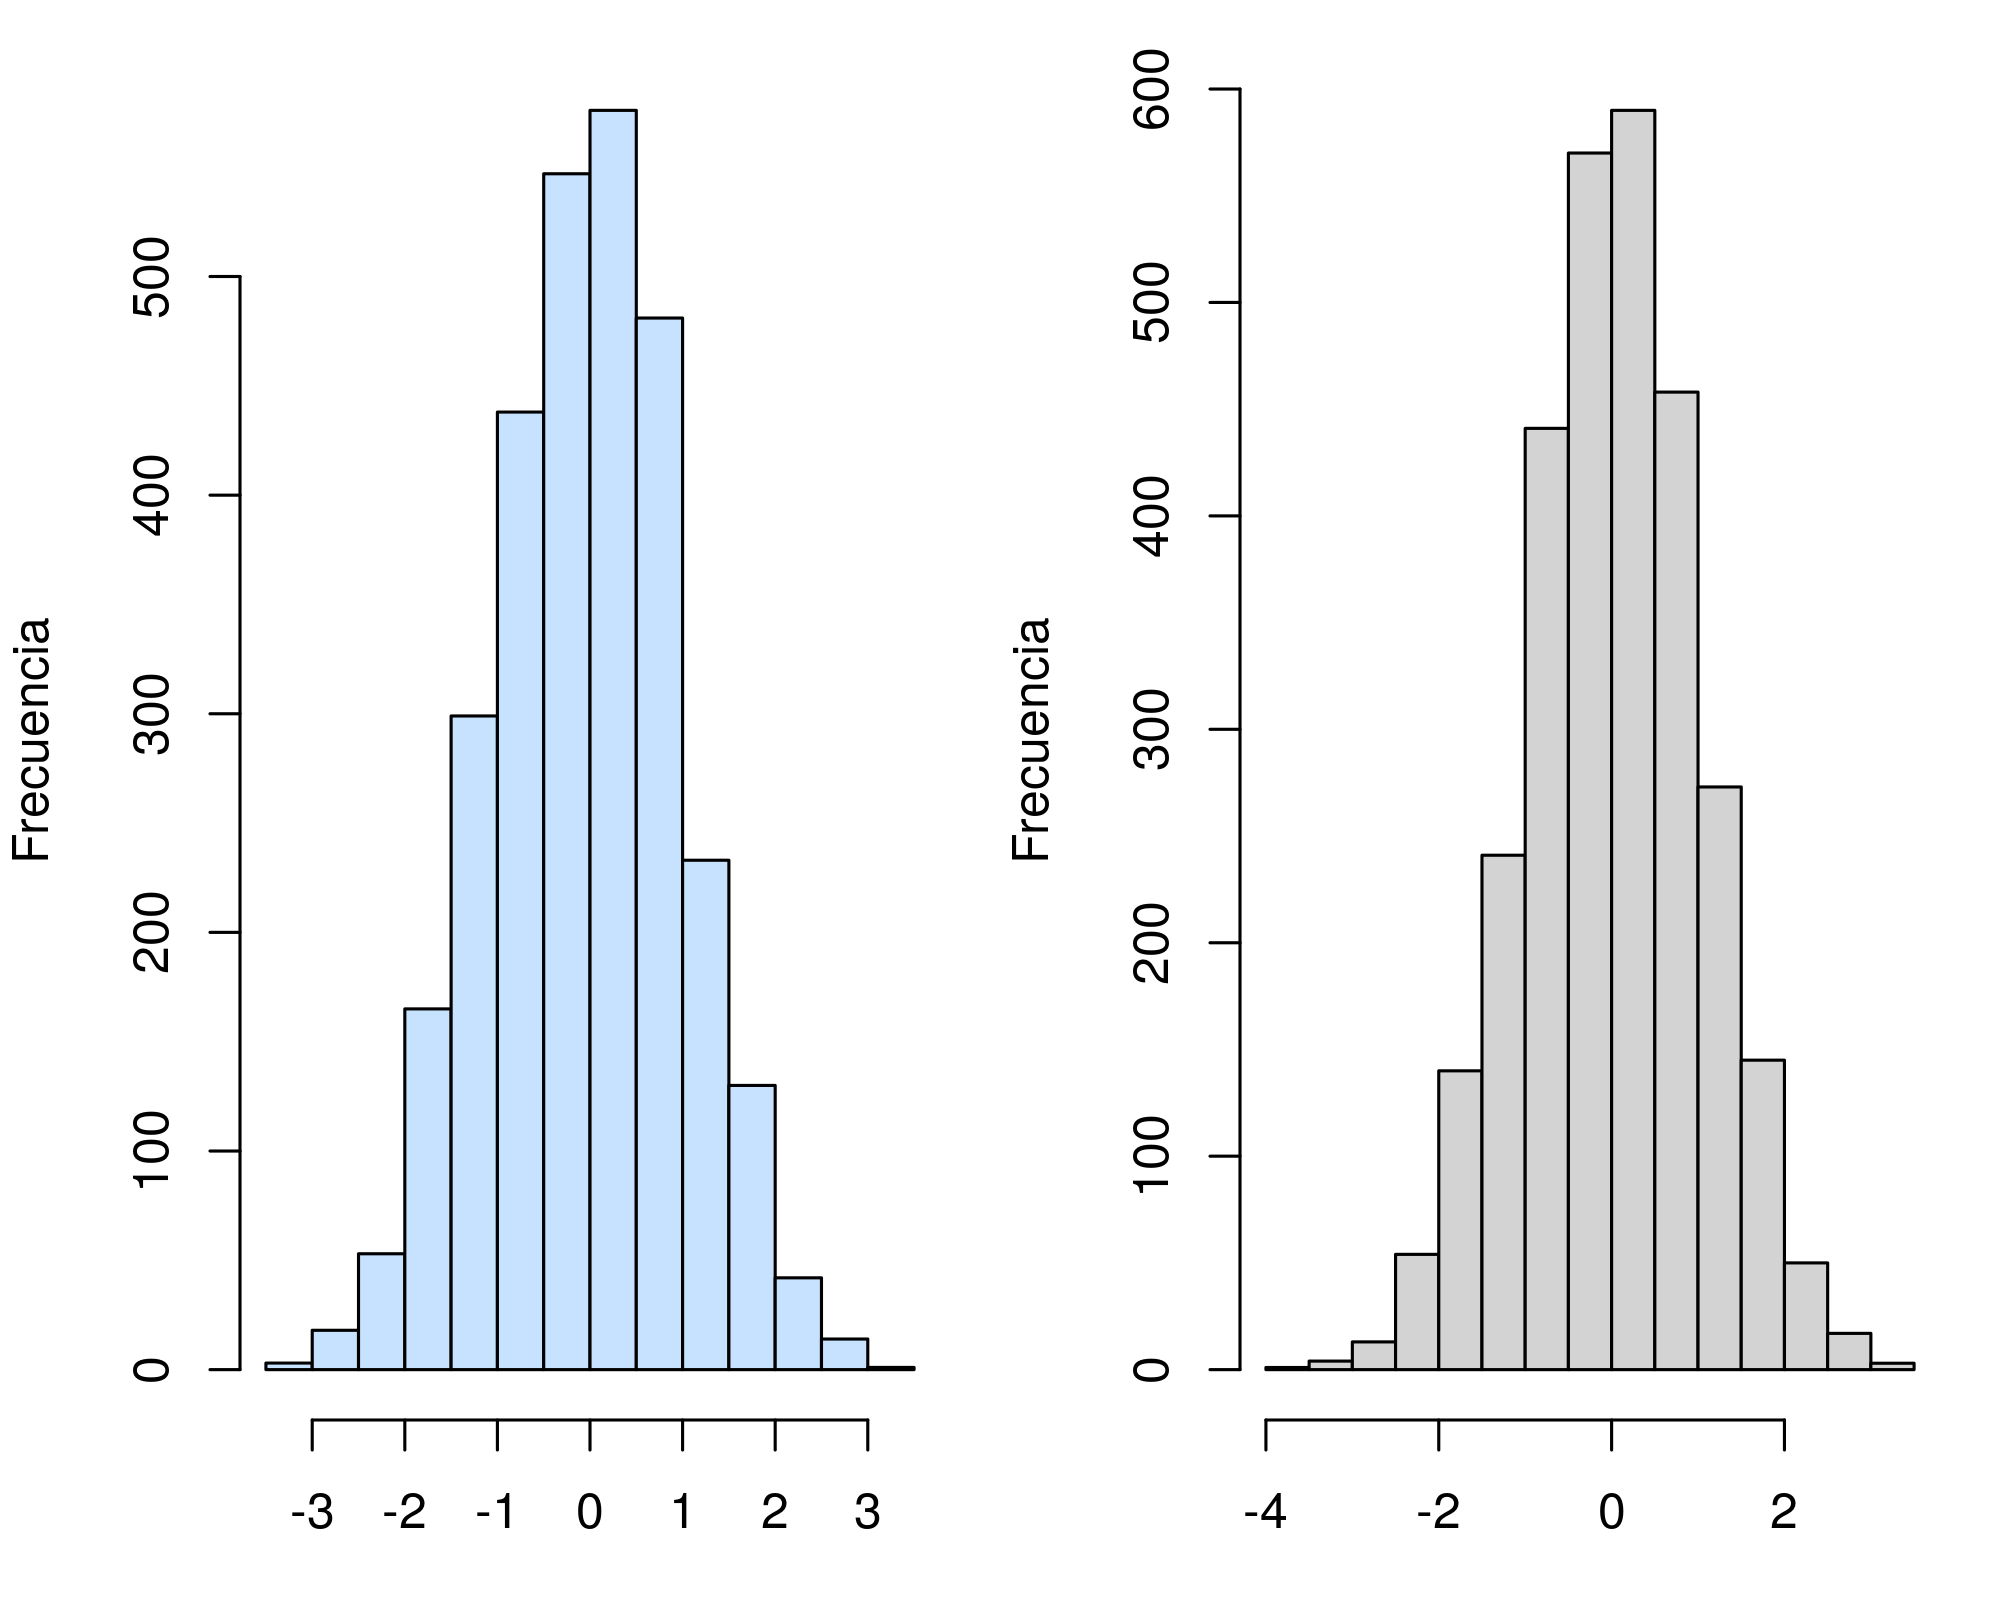
\includegraphics[width=0.6\textwidth]{normal_uniforme_regular.png}
		\caption{Distribución normal. En azul, la distribución generada por el método de Box-Muller usando el generador lineal congruencial con parámetros ``buenos'' y en gris la distribución generada por \texttt{rnorm(n)}.}
		\label{normal_bueno}
	\end{figure}
	
	Los resultados del $p$-valor al aplicar la prueba de normalidad a las diez réplicas se muestran en el cuadro \ref{pvalor-normal-bueno}. De las diez réplicas, unicamente dos no pasaron la prueba de normalidad. 
	
	\begin{table}
	\centering
	\caption{Resultados del $p$-valor al aplicar la prueba de {\em Shapiro} a los datos generados con \texttt{uniforme.R}.}
	\label{pvalor-normal-bueno}
	\begin{tabular}{rr}
		\hline
		Réplica & $p$-valor \\
		\hline
		1 &  0.167831102 \\
		2 & 0.722710035 \\
		3 &  0.388615457 \\
		4 &  0.193132625 \\
		5 &  0.001657073 \\
		6 &  0.407205524 \\
		7 &  0.174958154 \\
		8 &  0.683738471 \\
		9 &  0.016105365 \\
		10 & 0.189060094 \\
		\hline
	\end{tabular}
\end{table}
	

\bibliographystyle{plain}
\bibliography{biblio}

\end{document}

